%------------------------------------------------------------------------
%                       DISCUS COMMON Users guide
%------------------------------------------------------------------------

\documentclass[11pt]{report}

\usepackage[letterpaper]{geometry}
\geometry{height=8.5in}
\geometry{bottom=1.1in}
\geometry{left=1.1in}
\geometry{right=1.1in}

\usepackage[dvips]{graphicx}
\usepackage{fancyhdr}
\usepackage{floatflt}
\usepackage{tabularx}
\usepackage[round]{natbib}
\usepackage[hang,small,bf]{caption}
\usepackage{fancyvrb}
\usepackage{scalefnt}
\usepackage{color}
\usepackage{url}
\usepackage{hyperref}

\usepackage[T1]{fontenc}
\usepackage{palatino}

% General page style

\pagestyle{fancy}
\fancyhf{}
\fancyhead[L]{\bfseries \slshape\leftmark}
\fancyhead[R]{\bfseries Reference Guide}
\fancyfoot[R]{\bfseries Page \thepage}
\fancyfoot[L]{\bfseries \Discus Package}
\renewcommand{\footrulewidth}{0.4pt}
\renewcommand{\headrulewidth}{0.4pt}

\newcommand{\version}{5.30}

\newcommand{\discus}{\textsc{Discus}}
\newcommand{\Discus}{\textsc{Discus\ }}
\newcommand{\Diffev}{\textsc{Diffev\ }}
\newcommand{\diffev}{\textsc{Diffev}}
\newcommand{\Kuplot}{\textsc{Kuplot\ }}
\newcommand{\kuplot}{\textsc{Kuplot}}
\newcommand{\Mixscat}{\textsc{Mixscat\ }}
\newcommand{\mixscat}{\textsc{Mixscat}}
\newcommand{\Refine}{\textsc{Refine\ }}
\newcommand{\refine}{\textsc{Refine}}
\newcommand{\Suite}{\textsc{Discus Suite\ }}
\newcommand{\suite}{\textsc{Discus Suite}}


% Style for chapter start pages ..

\fancypagestyle{plain} {
  \fancyhf{}
  \fancyhead[R]{\bfseries Reference Guide}
  \fancyfoot[L]{\bfseries \Discus Package}
  \fancyfoot[R]{\bfseries Page \thepage}
  \fancyfoot[L]{\bfseries \Diffev \version}
  \renewcommand{\headrulewidth}{0.4pt}
}

% MacVerbatim style for macros

\definecolor{DarkBlue}{rgb}{0.1,0.0,0.5}

\DefineVerbatimEnvironment%
{MacVerbatim}{Verbatim}
{fontfamily=courier,
 fontsize=\scriptsize,
 fontseries=b,
 formatcom=\color{DarkBlue}}

\graphicspath{{pic/}}

\setlength\parindent{0pt}

%------------------------------------------------------------------------

\begin{document}

%------------------------------------------------------------------------
% Title
%------------------------------------------------------------------------

\begin{titlepage}
\begin{flushright}

  \hrule
  \vspace{15mm}
  \textbf{{\scalefont{8} \discus}} \\
  \vspace{5mm}
  \textbf{{\scalefont{4} Package}} \\
  \vspace{10mm}
  \textbf{{\Huge Reference Guide}} \\
  \vspace{10mm}
  \textbf{{\Huge Version  \version}} \\
  \vspace{10mm}

  \hrule
  \vspace{45mm}
  \textbf{developed by} \\

  \vspace{5mm}
  \textbf{\Large Reinhard Neder} \\
  Email: reinhard.neder@fau.de \\

  \vspace{ 2mm}
  \textbf{\Large Thomas Proffen} \\
  Email: tproffen@ornl.gov \\

  \vspace{12mm}
  \textbf{\Large 
     \url{http://tproffen.github.io/DiffuseCode/} 
  } \\

  \vspace{3mm}
  \hrule
  \vspace{3mm}
 
  \textit{Document created: \today}
\end{flushright}

\end{titlepage}

%------------------------------------------------------------------------
% Table of contents
%------------------------------------------------------------------------

\tableofcontents

%------------------------------------------------------------------------
% Short summary of the DISCUS package
%------------------------------------------------------------------------

\newpage
\chapter{Welcome} \label{welc}

Congratulations for downloading the \Discus package. The \Discus package
consists of the following programs:

\begin{itemize}
  \item \textbf{\textsc{DISCUS SUITE}}: The \Suite is a common program
  that includes the sections \Discus \Diffev \Refine and \kuplot. 
  It allows to switch
  seamlessly between the individual sections and will eventually replace
  the individual parts. It also offers an optimization for large scale 
  computing facilities. 

  \item \textbf{\textsc{DISCUS}}: This is the main diffuse scattering
  and defect structure simulation section. This is the section that
  gave the package its name.
  
  \item \textbf{\textsc{DIFFEV}}: This is a more recent addition. This
  section allows the refinement of a set of high level parameters 
  (\textit{e.g.} input parameters of a \Discus macro) based on a
  differential evolutionary algorithm.
  
  \item \textbf{\textsc{REFINE}}: This is newest addition to the 
  \Discus package. This section section allows a classical 
  least squares refinement. 
  
  \item \textbf{\textsc{KUPLOT}}: This is plotting section of the
  package. It is nearly as old as \Discus itself. 

  \item \textbf{\textsc{MIXSCAT}}: This part has been retired.
  
%  \item \textbf{\textsc{PDFFIT}}: This is a PDF refinement program.
%  It has been retired and users are encouraged to download the new
%  version \textsc{PDFgui} at \url{http://www/diffpy.org}.
\end{itemize}

Each of the sections has its own users guide which include disclaimers 
and the appropriate references to cite in case you are publishing work
derived from using these programs.

This manual contains a description of the command language common to all
programs as well as detailed installation instructions. \Discus itself 
has been developing over the last nearly 30 years and the command language
was developed before anyone knew about things like python. The commands
are loosely related to FORTRAN77 syntax, so the older generation should
have no trouble with it. 
\par
\ \par
Please visit the \Discus homepage frequently at  \\
\url{http://tproffen.github.io/DiffuseCode/} \\
and also consider subscribing 
to the \Discus mailing lists.

\section{Getting started} \label{start}

\subsection{Windows} \label{start-win}

Once the programs have been installed you should see an icon for each of 
the programs on your personal desktop. Double click the icon to start
the program of your choice.

At program start, the \Suite sets its starting folder to\\
\begin{MacVerbatim}
   C:\Users\your_name
\end{MacVerbatim}
where {\tt your\_name} will be your user name. The string {\tt Users}
may be slightly different depending on the language settings.
To work with data and macros that are stored in a separate folder, 
you need to change to this folder.

Within the \Suite program window, type the command {\tt cd } including a
blank space after the {\tt cd}. At this point do not hit the enter key.
Open the desired folder with the Windows-Explorer. Left click on the 
small folder symbol in the top line that indicates the path to your
folder. This should highlight the full path to the folder. 

Select the highlighted path to the folder
with CTRL-c. Activate the \Suite window and press the 
middle button on the mouse. This should place the full path into the
program window. 

Once you activate the window and hit the ENTER key the program will 
work in this folder.

\subsection{Linux} \label{start-linux}

Once you have installed the Diffuse program package, the binaries will
usually reside in the directory: {\tt /usr/local/bin/}. 
To use any of the programs, open a terminal window, switch to the 
desired directory and type {\tt discus\_suite}.

Several command line options are available for the Linux version.
The most important one is to start the execution of a macro:

\begin{MacVerbatim}
discus_suite -macro useful.mac  
discus_suite -macro useful_with_params.mac  par1 par2 par3
\end{MacVerbatim}

The first line would start \Suite and begin the automatic execution
of macro {\tt useful.mac}. Likewise in the second line, the macro
{\tt useful\_with\_params.mac} is started, which takes three parameters.
The actual strings that
you provide for <par1>, <par2>, <par3> are handed down as parameters to 
this macro. Note that there are no comma between the parameters.

For info on further command line options the the on-line help for
the Command language.

\subsection{MacOS} \label{start-MAC}
Once you have installed the Diffuse program package, the binaries will
usually reside in the directory: {\tt \${HOME}/bin/}.  
To use \Suite open the {\tt terminal} app switch to the desired
directory snd type {\tt discus\_suite}.

The command line options are identical to the \ref{start-linux} Linux version.


\section{Command language overview} \label{over}

All sections of the \Suite are controlled by a command language. The
basic command style is a command verb that may be accompanied by one 
or several parameters. You must type at least one empty space between
the command and the list of parameters. The parameters are all 
separated from each other by a comma as in the following short example: 

\begin{MacVerbatim}
  discus
  ! a comment
  # another comment
  read
  cell example.cell, 2,3, 4
  show atom, all   ! In line comment after exclamation mark
  exit
\end{MacVerbatim}

Anything to the right of an exclamation mark {\tt !} or a hash tag
{\tt \#} is considered a comment and is not interpreted. 

Most commands can be abbreviated, as long as the short form is
still unique. Thus these commands are all valid forms to 
step into the \Discus fourier menu:

\begin{MacVerbatim}
  fourier
  fourie
  fouri
  four
  fou
\end{MacVerbatim}


Several command throughout the \Suite take optional parameters.
Sometimes these are the last parameter(s) that you can simply
omit. See the on-line help for the individual commands for
full information.

More and more though the optional parameters are specified with the
syntax: Name of the optional parameter, a colon ":" and the actual
value you want to provide:
\begin{MacVerbatim}
 run  plot:inter, kill:yes
\end{MacVerbatim}
If an optional parameter is omitted, its value goes back to the
default value. This is a bit different compared to the
non-optional parameters. These parameters retain their value
until you change the value explicitly.

As the named optional parameters are identified by their name,
they may be given in arbitrary order.

As the most efficient alternative to the interactive input of
commands by the user, the \Suite works best when you place all the
commands into one or more simple text files, referred to as macros.
All sections of the \Suite can read these and execute the commands within
such a macro file as if they had been typed interactively at the prompt.

See the section {\ref {mac}} for more details. A particular macro called
{\tt autorun.mac} will be executed automatically at program start.

Besides the {\tt autorun.mac} at Linux and MacOS you can use command
line options {\ref {cmdopt} to start a macro at program start. 

\subsection{Help} \label{over-help}

The \Suite offers the manuals, and on-line help. To access any of the 
manuals from the \suite, type :
\begin{MacVerbatim}
  manual                 ! Opens the manual for your current section
  manual section:suite   ! Opens the SUITE manual
  manual section:discus  ! Opens the DIFFEV manual
  manual section:refine  ! Opens the REFINE manual
  manual section:diffev  ! Opens the DISCUS manual
  manual section:kuplot  ! Opens the KUPLOT manual
  manual section:package ! Opens this PACKAGE manual
\end{MacVerbatim}

The \Suite will open the manual with a standard PDF viewer. Alternatively
you can open the manual with your favorite viewer with the second 
optional parameter, for example:
\begin{MacVerbatim}
 manual section:package, viewer:qpdfview
\end{MacVerbatim}
where the {\tt viewer\_name} shall be replaced by your favorite.

At a Linux system the manual files are usually installed into 
{\tt /usr/local/share}.

At a Windows system the manual files are in the {\tt share} folder 
within the Discus installation, commonly at
{\tt c:Program Files (x86)\textbackslash Discus\textbackslash share}.  

On-line help is available for each command through the {\tt help}
command. A straight {\tt help} will open the on-line help at the
current section respectively menu within a section. Alternatively
you can migrate immediately to the on-line help for a specific 
command by adding the command name after the help command. If 
the command is within a menu of your current section you can 
access the help by providing the menu as first parameter, followed
by the command name.

\begin{MacVerbatim}
help               ! Opens the help at the current section / menu
help fourier       ! Opens the help for the fourier command
help fourier, lots ! Opens the help for the fourier> lots command
\end{MacVerbatim}

To leave the on-line help simply hit the {\tt ENTER} key. At each 
help level the on-line help gives a list of further topics, type
any of these names to get help on one of these topics. 

The help is organized hierarchically for the menus. At the \Discus
section for example the top level provides help to all \Discus
commands. If you step into the help of (for example) the 
{\tt fourier} menu you can access the {\tt fourier} commands. 

To go back to an upper help level type {\tt ..} at the 
on-line help prompt.

As most help entries are lengthy, the list of help options at
the current level will have moved out of your view. Just type
{\tt ?} to refresh this list.

\subsection{Main commands} \label{over-main}

The main \Suite commands are summarized in table \ref{over-cmds}
followed by a list of common Unix commands.

\begin{table}[!tbh]
\centering
\begin{tabularx}{\textwidth}{|p{50mm}|X|}
  \hline
  {\bf Name} &  {\bf Description} \\
  \hline\hline
  discus & Go from the main \suite level to the \Discus
           section.
           Leave this section with an "exit" command. \\
  \hline
  diffev & Go from the main \suite level to the \Diffev
           section.
           Leave this section with an "exit" command. \\
  \hline
  kuplot & Go from the main \suite level to the \Kuplot
           section. 
           Leave this section with an "exit" command. \\
  \hline
  branch <name> & Step sideway from your current section into 
           the section <name>. 
           Leave this section with an "exit" command. \\
  \hline
  exit & Leave a menu, a section or the program. If you are 
         within a menu of any of the three sections, you will
         get back to the main level of this section. If you are
         at the top level of any of the three sections, you 
         will get back to the main \Suite level. If you are at
         the main\Suite level, the program will terminate 
         without further confirmation. \\
  \hline
   help & Enter the help menu\\
  \hline
   @macro.mac & Run the commands in file "macro.mac" as if 
          they were typed interactively. See section \ref{mac}
          for full details.\\
  \hline
   learn macro.mac & Start to learn everything to type and
          log these command into the file "macro.mac". 
          This log will include everything you type, including 
          errors...\\
  \hline
   lend & Finish the learn sequence. The macro "macro.mac is 
          now available to be run as {\tt @macro.mac}\\
  \hline
   cd <folder> & Change the directory / folder to the new 
          directory / folder <folder>. 
          The path can be a 
          relative path as in {\tt cd ../new\_folder} or
          an absolute path.\\
  \hline
   system <command> & Instruct your operating system to execute
          the command <command>. As the \Suite is really a
          Unix driven program, even on a Windows computer
          these are predominantly Unix commands. Some 
          commonly used commands are listed in Table
          \ref{over-unix}\\
  \hline
   set error, <status> & The <status> may be "continue", 
          "exit" "live".\\
  \hline
   show  & Most sections and menus offer a "show" command
           to display the local settings. Check the on-line
           help at the respective menu for details.\\
  \hline
   run   & Most of the menus expect several commands that
           define the simulation / calculation prior to the
           calculation. The actual 
           calculation is carried out with the "run" command
           at the respective menu.\\
  \hline
   set prompt, <status> & The <status> may be "on", "off".\\
  \hline
   update & Available at the main\Suite level, this command 
            will update the \Suite to run the latest release.\\
  \hline
\end{tabularx}
\caption{\label{over-cmds}Main \Suite commands}
\end{table}

The \Suite can react in different ways to an erroneous calculation or 
erroneous input. The default "continue" is to display an error message 
and to stop the execution of a macro/calculation. Thereafter the program 
continues with the regular interactive prompt. Sometimes one may
want to live on after a fault. This may for example occur if you test
for the existence of a file or directory/folder, or if you encounter 
the end of file upon a read. A macro can live on if the error status is
set to "live". The most stringent reaction to an error is to terminate
the  \Suite with the error status "exit". Keep in mind that no data are
saved!

During a regular interactive session the program displays a prompt like
\begin{MacVerbatim}
suite>         ! Prompt within the top level suite
discus/four>   ! Prompt within a sub menu of a section, here DISCUS
\end{MacVerbatim}
If a macro is executed, the lines that the \Suite reads from the macro
file are also echoed to the screen. This may produce lengthy output.
The choices offered are to set the prompt "on" or "off". An optional
parameter allows to save the current prompt status so that the "old" 
status can be restored at a later stage.


\begin{table}[!tbh]
\centering
\begin{tabularx}{\textwidth}{|p{50mm}|X|}
  \hline
  {\bf Name} &  {\bf Description} \\
  \hline \hline
   pwd & Inquire the current directory/folder, the
          {\bf p}resent {\bf w}orking {\bf d}irectory.\\
  \hline
   ls    & List the content of the current directory/folder\\
  \hline
   mkdir <folder> & Make the new directory/folder <folder> \\
  \hline
   mkdir -p <folder> & Make the new directory/folder <folder>,
         including any intermediate parent folders. 
         This command version will not flag an error,
         if the folder does already exist. \\
  \hline
   rm <filename> & Remove the file <filename>. \\
       & Careful, this command does not ask for 
         a confirmation! \\
       & If the file does not exist
         or if it is a protected file you will get an
         error message.\\
  \hline
   rm -f <filename> & Forced remove the file <filename>. \\
       & Careful, this version does not ask for a confirmation!\\
       & This command version will not flag an error,
         if the file does not exist. \\
  \hline
   cp <from> <to> & Copies the old file <from> to a new name and
         or directory/folder <to>.\\
  \hline
\end{tabularx}
\caption{\label{over-unix}Common Unix commands}
\end{table}

Most of the Unix commands offer many more options. Just try it 
out, in many cases a parameter like "-help" 
or "--help" will give a short summary of the available options.
Examples:

\begin{tabularx}{\textwidth}{p{25mm}X}
ls -a & List all files, that includes hidden files\\
ls -l & List a long listing that includes many details\\
ls -R & List recursively into sub directories as well\\
\end{tabularx}

Unix offers many possibilities to work in a flexible manner with file 
names. You can place into the filename different {\it wild} characters:

\begin{tabularx}{\textwidth}{p{25mm}X}
* & character string of any length\\
? & exactly one character\\
\ [a-z,A-Z] & a character from interval a-z or A-Z.\\
\end{tabularx}

You may provide a single interval as well, and also a range of numbers.
Examples:

\begin{tabularx}{\textwidth}{p{25mm}X}
ls *.mac & List all files that end in ".mac"\\
ls data.0[0-9]1 & List all files called data.001, data.011, to data.091
files called data.002 etc. are omitted\\
\end{tabularx}


\subsection{Interrupt} \label{over-inter}
If a lengthy calculation or macro appears to be faulty you can interrupt
the calculation with a {\tt CTRL-c}. The \Suite will offer a selection
how to proceed after this interrupt. You can:


\begin{tabularx}{\textwidth}{p{25mm}X}
{\tt resume} & the calculation. The program will (hopefully) resume
   the calculation as if nothing had happened. \\
{\tt continue} & with the normal interactive prompt. At this point
   you will be at the top level of the \Suite. Be aware that a macro
   may have changed the folder/directory. You are well advised to 
   check this with a command {\tt system pwd} \\
{\tt save} & The program will write the current crystal 
   to a file {\tt EMERGENCY.STRU} to give you a chance to recover 
   (most) of your work. It then continues in the same fashion as with the
   continue command. \\
{\tt exit} & the \Suite. \\
\end{tabularx}
%
%------------------------------------------------------------------------
%

\section{Parallel computing } \label{parallel}

The \suite uses parallel computing in two very different fashions. For a 
long tim \diffev is run effectively in parallel, see the \diffev manual for 
details.

As of version 6.02 the \suite has also been compiled with openMP, a standard 
for parallel processing. The parallel processing is done automatically and 
usually does not require user input. 

As of version 6.02 the parallel processing is used to accelerate the calculations
of a powder diffraction pattern, a single crystal Fourier, and the Monte-Carlo
simulations. More to come. 

At startup \suite will check how many physical and logical cores are available 
at the computer. Many modern CPU's provide the capability to run two processes
in {\it parallel} on the same physical CPU, a term referred to as hyperthreading. 
This will be advantageous, if one of the two processes is for example waiting for 
external signals. If the \suite uses two thread in parallel on the same 
physical core, the administrative overload will actually slow down the  computing 
and no performance increase is obtained. At startup \suite thus limits the 
number of parallel threads to the number of phycsical units. 

Two commands relate to parallel processing via openMP. The command
{\tt show parallel} will display the number of threads currently used as well
as the number of physical and logical cores available. 

With {\tt set parallel} you can determine how many threads to use in paralleli
computations. See the on-line help for more details on these two command.
%
%------------------------------------------------------------------------
%
%------------------------------------------------------------------------
% Chapter:  FORTRAN interpreter
%------------------------------------------------------------------------

\chapter{FORTRAN style interpreter \label{fort}}

The programs include a FORTRAN style interpreter that allows the
user to program complex modifications.  The interpreter provides
variables, linked to data sets and free variables, loops, logical
construction, basic arithmetic and built in functions.  Commands
related to the FORTRAN interpreter are {\tt =, break, do, else,
elseif, enddo, endif, eval, if} and {\tt variable}. The command {\tt
eval} allows to examine the contents of a variable or to evaluate an
expression, e.g. {\tt eval r[1]*0.5}. \par

%------------------------------------------------------------------------

\section{Variables \label{var}}

The programs in the {\it DISCUS} suite use variables to store 
data. The programs distinguish three types of variables:
\begin{itemize}
  \item Variables with fixed name for general use
  \item Variables with user defined names for general use
  \item Variables with fixed name that carry program information
\end{itemize}

{\bf Variables with fixed name for general use}

There are two types of variables: variables of type integer or real, 
denoted by their fixed names "i" and "r", immediately followed by a left square bracket [, 
one or more indices (separated by a comma), and finally a right square bracket ]. 

Examples for build in variables are given next.

\begin{quote}
  {\it Example :\/} i[1], r[0], i[i[1]], x[2]
\end{quote}

The build-in variables {\tt i[n]} and {\tt r[n]} are general purpose 
variables. The index {\tt n} can take integer values from zero to a 
maximum value defined at program compilation, usually 500. In addition,
 each of the program has a number of build-in
variables related to its function. \Discus for example has a number of 
variables related to the structure that the user is using, like unit cell 
dimensions, atom positions etc. For a list of these variables,
please refer to the respective program users guides.
\par
\par

{\bf Variables with user defined names for general use}\\
The second set of variables are single valued variables with user
defined names. These allow the user to use more obvious variable 
names. The programs allow to define real valued, integer valued
and character variables.
With almost identical syntax, the user can provide 1-D and 2-D
integer and real valued arrays. Currently no Character arrays are provided.

An example of the use of defined variables is shown here:
%
\begin{MacVerbatim}
   1  variable real,alpha,90.0
   2  variable real,beta
   3  variable real,diff
   4  beta = 94.0
   5  diff = alpha - beta
   6  eval diff
\end{MacVerbatim}
%
In line one we define a real variable {\tt alpha} with an initial
value of 90. Next, two more variables are defined and the difference
between {\tt alpha} and {\tt beta} is calculated (line 5) and the
result displayed on the screen (line 6). 

Recently another type of variables was added to the command language:
character variables. These can be used in conjunction with format 
statements (see command reference under \textit{expressions}). An example 
setting the plot title in \textsc{Kuplot} to the current date is listed
below.
%
\begin{MacVerbatim}
   1  variable character,datum
   2  #
   3  datum="%c",fdate(0)
   4  tit2 "Plotted on %c",datum
\end{MacVerbatim}
%
Note the slightly different way character intrinsic functions are used.
A complete list of character functions can be found in Table
\ref{func-char}.

To define 1-D or 2-d arrays, simply add the optional parameter "dim"
to the variable definition.
\begin{MacVerbatim}
   1  variable real, mat_a, dim:[3:3]
   2  variable real, vec_a, dim:[3]
\end{MacVerbatim}

To work on user supplied matrices, the \Suite provides several commands:
\begin{itemize}
  \item matmul: Multiply matrices
  \item matadd: Add      matrices
  \item detmat: Calculate the determinant
  \item mattrans: Calculate the transposed matrix
\end{itemize}
%
\par

{\bf Variables with predefined name }\\

Starting with version 5.7.0 system wide variables with fixed name 
were introduced. Currently these are mostly related to the refinement,
see the \Diffev manual for details. 

The general predefined variables are explained in the following list:

\begin{itemize}
  \item UNDEF = -1  A status is undefined
  \item TRUE  = 1   A status is true
  \item FALSE = 0   A status is false
  \item IS\_TOP = 0 Possible value for STATE, if you are currently at the
                    top program level. This will be the case within the
                    suite. If the individual programs DISCUS, KUPLOT
                    or DIFFEV are used as stand alone programs you will 
                    be in a STATE=IS\_TOP in their main menu.
  \item IS\_SECTION = 1  Possible value for STATE, if you are currently at
                    one of the three sections DISCUS, DIFFEV, KUPLOT
                    within the suite.
  \item IS\_BRANCH = 2  Possible value for STATE, if you are currently in
                    a section after a "branch" command. 
  \item SUITE = 0   Possible value for PROGRAM, if you are within the suite.
  \item DISCUS = 1   Possible value for PROGRAM, if you are within discus.
  \item DIFFEV = 2   Possible value for PROGRAM, if you are within diffev.
  \item KUPLOT = 3   Possible value for PROGRAM, if you are within kuplot.
  \item MPI\_OFF = 0 Possible value for MPI, if the program was not started
                     with mpi.
  \item MPI\_ON  = 1 Possible value for MPI, if the program was started
                     with mpi.
  \item PROGRAM      Receives a value of (SUITE, DISCUS, DIFFEV, KUPLOT)
                     depending on which part you are currently within.
  \item STATE        Receives a value (IS\_TOP, IS\_SECTION, IS\_BRANCH),
                     depending on the way this section was entered.
  \item MPI\_FIRST   Relevant to \Diffev only. The value will be UNDEFined
                     in the other sections. Within \Diffev it tells a 
                     slave program if the slave was invoked as the first
                     'run\_mpi' command within the current refinement generation.
  \item MPI          Receives a value of MPI\_OFF or MPI\_ON. 
  \item PI           Pi = 3.1415... 
\end{itemize}  

One further system variable is {\tt PI}. The capitalization is mandatory.

{\bf Variables with fixed name that carry program information}

These variables, which are common to the whole program suite are 
used by the programs to return information to the user.

Currently just one such variable {\tt res[n]} exists. It is used
in a wide variety of commands and functions to return a successful
operation or to contain result values.

As an example see:
%
\begin{MacVerbatim}
   1  fexist dummy.file
   2  eval res[0]
   2  eval res[1]
\end{MacVerbatim}
%
Here the {\tt res} variable is used to flag the existence of the file
called "dummy.file". {\tt res[0]} usually carries the number of 
results returned, in this special case one. Here {\tt res[1]} would
be equal to one if the file exists and zero if it does not exist.


%------------------------------------------------------------------------

\section{Arithmetic expressions \label{arith-exp}}

The language allows the use of arithmetic expressions using the same
notation as in FORTRAN. Valid operators are {\tt +, -, *, /} and
for the exponentiation {\tt **}. Expressions can be grouped by 
round brackets ( and ). The
usual hierarchy for the operators holds. Values of expressions can
be assigned to any modifiable variable. If you know FORTRAN (or
another programming language) you will have no problems with these
examples.

\begin{quote}
  i[0] = 1 \\
  r[3] = 3.1415 \\
  r[i[1]] = 2.0*(i[5]-5.0/6.5)
\end{quote}

%------------------------------------------------------------------------

\section{Logical expressions \label{log-exp}}

Logical expressions are formed similar to FORTRAN. They may contain
numerical comparisons using the syntax: {\it $<$arithmetic
expression$><$operator$><$arithmetic expression$>$}. The allowed
operators are 

{\tt <, <=, >, >=, ==, /=}

or in the older Fortran77 style:

{\tt .lt., .le., .gt., .ge., .eq., .ne.} 

for operations less than, less equal, greater than,
greater equal, equal and not equal, respectively. Logical
expressions can be combined by the logical operators:

 {\tt .not., .and., .or., .xor., .eqv.}.

The following example shows an
expression that is true for values of {\tt i[1]} within the interval
of 3 and 11, false otherwise.

\begin{quote}
  i[1] >= 3 .and. i[1] <= 11 \\
  i[1].ge.3 .and. i[1].le.11
\end{quote}

Logical operations may be nested and grouped using round
brackets ( and ). For more examples see section \ref{if}.

%------------------------------------------------------------------------

\section{Character expressions\label{char-exp}}

Character expressions allow you to write annotations in \kuplot, nicely 
formatted comments in the output of any section or complex filenames.

The first use might be that of character variables within the sections 
of the \Discus suite. The simplest assignment of values to a character 
variable takes the form:
\begin{MacVerbatim}
  character variable, string
  string = 'This is a string'
\end{MacVerbatim}

In order to concatenate strings, or to place numerical values into a 
string three format specifiers are provided:

\begin{MacVerbatim}
  "%c"   or "%10c"
  "%d"   or "%10d"
  "%f"   or "%10.4f"
\end{MacVerbatim}

All specifiers require the leading {\tt \%} as control character. 
The {\tt \%c} specifier allows to place the value of a character value or 
a character string into the expression. A number between the {\tt \%} and 
the {\tt c} signifies the width of the string that will be placed. If the 
incoming string is too long it will be truncated as in the following 
examples:
\begin{MacVerbatim}
  character variable, string
  character variable, line
  string = 'abcdefghij'
  line   = "%c", string    ! place at variable length 
  echo "%c",line
  abcdefghij               ! This will be shown on screen
  line   = "%c5", string   ! place as 5 character long string
  echo "%c",line
  abcde                    ! This will be shown on screen
  line   = "%5c", string(4:8)  ! take a sub string 
  echo "%c",line
  defgh                    ! This will be shown on screen
\end{MacVerbatim}

The {\tt \%d} specifier allows to write the value of an integer expression
into a character string. The optional number between the {\tt \%} and the 
{\tt d} specifies the number of digits that will be printed. If a 
capital {\tt D} is used in combination with the the width defining 
number, any leading digits are printed as zeros.

\begin{MacVerbatim}
  echo "%d more %d", 1, 2
  1 more 2                ! This will be shown on screen
  echo "%4D more %4d", 1, 2
  0001 more    2          ! This will be shown on screen
\end{MacVerbatim}

The {\tt \%f} specifier allows to write the value of a real valued expression
into a character string. The optional number between the {\tt \%} and the 
{\tt f} specifies the width of the field printed and the number of 
digits that follow the decimal point. If a  
capital {\tt F} is used in combination with the the width defining
number, any leading digits are printed as zeros.

\begin{MacVerbatim}
  echo "%f more %d", 1.1, 20.2
  1.000000 more 20.0000000 ! This will be shown on screen
  echo "%4.1F more %6.2f", 1.1, 20.2
  01.0 more   20.20        ! This will be shown on screen
\end{MacVerbatim}
%------------------------------------------------------------------------
%------------------------------------------------------------------------

\section{Intrinsic functions \label{func}}

Several intrinsic functions are defined.  Each function is
referenced, as in FORTRAN, by its name followed by a pair of
parentheses ( and ) that include the list of arguments. The ( does
not have to immediately follow the function name.  Trigonometric and
arithmetic functions are listed in table \ref{func-trig}.  Table
\ref{func-ran} contains various random number generating functions.
Some programs such as \Discus have a set of specific intrinsic 
functions allowing one to for example calculate bond length. Again 
each individual users guide will contain a table of these specific
functions.

\begin{table}[!tbh]
\centering
\begin{tabularx}{\textwidth}{|p{12mm}|p{45mm}|X|}
  \hline
  {\bf Type} & {\bf Name} & {\bf Description} \\
  \hline\hline
  real & sin(r) cos(r) tan(r) &
         Sine, cosine and tangent of $<$r$>$ in radian \\
  real & sind(r) cosd(r) tand(r) &
         Sine, cosine and tangent of $<$r$>$ in degrees \\
  real & asin(r) acos(r) atan(r) &
         Arc sin, cosine, tangent of $<$r$>$, result in radian \\
  real & asind(r) acosd(r) atand(r) &
         Arc sin, cosine, tangent of $<$r$>$, result in degrees \\
  \hline
  real & sqrt(r) & Square root of $<$r$>$ \\
  real & exp(r) &  Exponential of $<$r$>$, base e \\
  real & ln(r) &   Logarithm of $<$r$>$ \\
  real & sinh(r) cosh(r) tanh(r) &
                   Hyperbolic sine, cosine and tangent of $<$r$>$ \\
  \hline
  real    & abs(r)      &  Absolute value of $<$r$>$ \\
  integer & mod(r1, r2) &  Modulo $<$r1$>$ of $<$r2$>$ \\
  integer & int(r)      &  Convert $<$r$>$ to integer \\
  integer & nint(r)     &  Convert $<$r$>$ to nearest integer \\
  real    & frac(r)     &  Returns fractional part of $<$r$>$ \\
  \hline
  real    & min(r1, r2) &  Smaller number of $<$r1$>$ and $<$r2$>$ \\
  real    & max(r1, r2) &  Larger number of $<$r1$>$ and $<$r2$>$ \\
  \hline
\end{tabularx}
\caption{\label{func-trig}Trigonometric and arithmetic functions}
\end{table}

\begin{table}[!tbh]
\centering
\begin{tabularx}{\textwidth}{|p{12mm}|p{30mm}|X|}
  \hline
  {\bf Type} & {\bf Name} & {\bf Description} \\
  \hline\hline
  real & ran(r) &         Uniformly distributed pseudo random number
                          between 0.0 inclusively and 1.0 exclusively.
                          Argument $<$r$>$ is a dummy\\
  real & gran(r1, typ) &   Gaussian distributed random number with mean
                          0 and a width given by $<$r1$>$. If $<$typ$>$
                          is "s" $<$r1$>$ is taken as sigma, if
                          $<$typ$>$ is "f" $<$r1$>$ is taken as
                          FWHM. \\
  real & gbox(r1, r2, r3) & Returns pseudo random number with
                          distribution given by a box centered
                          at 0 with a width of $<$r2$>$ and two half
                          Gaussian distributions with individual
                          sigmas of $<$r1$>$ and $<$r3$>$ to the left
                          and right, respectively. \\
  real & gskew(r1,typ) &  Skewed Gaussian distributed random number 
                          with mean
                          \\
  real & logn(r1,r2)      & Returns a lognormal distributed number
                          with mean $<$r1$>$ and sigma $<$r2$>$ of
                          the underlying
                          Gaussian distribution.\\
  integer & pois(r1)      & Returns a Poisson distributed random
                          number with mean $<$r1$>$.\\
  \hline
\end{tabularx}
\caption{\label{func-ran}Random number functions}
\end{table}

Finally the available functions returning a character string are
listed in Table \ref{func-char}.

\begin{table}[!tbh]
\centering
\begin{tabularx}{\textwidth}{|p{30mm}|X|}
  \hline
  {\bf Name} & {\bf Description} \\
  \hline\hline
  date(0)        & Returns current date as {\tt CCYYMMDDhhmmss.sss}.\\
  fdate(0)       & Returns current date as character string {\tt Day Mon dd hh:mm.ss yyyy}.\\
  fmodt(0)       & Returns modification date of the last file opened 
                   as character string {\tt Day Mon dd hh:mm.ss yyyy}.\\
  cdate(0)       & Returns current date as {\tt Day Mon DD hh:mm:ss CCYY}.\\
  getcwd(0)      & Returns the current working directory.\\
  getenv('VAR')  & Returns the value of the environment variable
                   {\tt VAR}.\\
  \hline
\end{tabularx}
\caption{\label{func-char}String functions}
\end{table}


%------------------------------------------------------------------------

\section{Intrinsic commands  \label{cmds}}

To operate on user variables that are 1-D or 2-D matrices, the \Suite 
provides a couple of standard operations. These are listed in Table \ref{cmds-cmds}:

\begin{table}[!tbh]
\centering
\begin{tabularx}{\textwidth}{|p{30mm}|X|}
  \hline
  {\bf Name} & {\bf Description} \\
  \hline\hline
  matmul         & multiplies two matrices or a matrix by a scalar  \\
  matadd         & Adds two matrices. The second matrix can be multiplied by a scalar. \\
  detmat         & Calculates the determinant of the input matrix and stores this in 
                   the output matrix. \\
  mattrans       & Calculates the transpose of the input matrix and stores this in 
                   the output matrix. \\
  \hline
\end{tabularx}
\caption{\label{cmds-cmds}Matrix commands}
\end{table}

%------------------------------------------------------------------------

\section{Loops \label{do}}

Loops can be programmed using the {\tt do} command.
Three different types of loops are implemented. The first type
executes a predefined number of times. The syntax for this type of
loop is

\begin{quote}
{\it do $<$variable$>$ = $<$start$>$,$<$end$>$ [,$<$increment$>$] \\
     \ldots commands to be executed \ldots \\
     enddo }
\end{quote}

Following modern Fortran, the word "enddo" may
also be spelled as "end do" with arbitrary blanks
between the words.

Loops may contain constants or arithmetic expressions for
$<$start$>$, $<$end$>$, and $<$increment$>$.  $<$increment$>$
defaults to 1.  The internal type of the variables is real.  The
loop counter is evaluated from {\it ($<$end$>$ -
$<$start$>$)/$<$increment$>$ + 1}. If this is negative, the loop is
not executed at all.  The parameters for the counter variable, start
end and increment variables are evaluated only at the beginning of
the do - loop and stored in internal variables.  It is possible to
change the values of $<$variable$>$, $<$start$>$ and/or $<$end$>$
within the loop without any effect on the performance of the loop.
This practice is not encouraged, could, however, be an unexpected
source of errors. \par

The second type of loop is executed while $<$logical expression$>$ is
true. Thus it might not be executed at all. The syntax for this type
of loop is

\begin{quote}
{\it do while $<$logical expression$>$ \\
     \ldots commands to be executed \ldots \\
     enddo }
\end{quote}

The last type of loop is executed until $<$logical expression$>$ is
true. This loop, however, is always executed once and has the
following syntax

\begin{quote}
{\it do \\
     \ldots commands to be executed \ldots \\
     enddo until $<$logical expression$>$ }
\end{quote}

In the body of commands any valid program commands can be used.
This includes calls to the sub levels, further do loops or macros,
even if these macros contain do loops themselves.  The maximum level
of nesting is limited by the parameter {\it MAXLEV} in the file {\it
doloop\_mod.f90}.  If necessary adjust this parameter to allow for deeper
nesting.  All commands from the first {\tt do} command to the
corresponding 'enddo' are read and stored in an internal array. This
array can take at most {\it MAXCOM} (defined in file {\it
doloop\_mod.f90} as well) commands at every level of nesting.  If lengthy
macro files are included in the do loop, this parameter might have
to be adjusted.  \par

If a do loop (or an if block) needs to be terminated, the {\tt
break} command will perform this function.  The parameter on the
{\tt break'} command line gives the number of nested levels of {\tt
do} and {\tt if} blocks to be terminated. The interpreter will
continue execution with the first command following the
corresponding {\tt enddo} or {\tt endif} command.  An example is
given below, note, that the line numbers are only given for better
orientation and are no actual part of the listed commands. \par

\begin{MacVerbatim}
     1  do i[2]=1,5
     2     do i[1]=1,5
     3        if ((i[1]+i[2]) .eq 6) then
     4           break 2
     5        endif
     6     enddo
     7  enddo
\end{MacVerbatim}

In this example, the execution of the inner do-loop will stop as
soon as the sum of the two increment variables {\tt i[1]} and {\tt
i[2]} is equal to 6.  The program continues with the {\tt enddo}
line of the outer do - loop.  Notice that two levels need to be
interrupted, the if block and the innermost do loop.  If the
parameter had been equal to one, only the if block would have been
interrupted, while the innermost do loop would have continued
without break.\par

%------------------------------------------------------------------------

\section{Conditional statements \label{if}}

Commands can be executed conditionally by using the {\tt if}
command. Analogous to FORTRAN, the if-control structure takes the
following form:

\begin{quote}
{\it if ( $<$logical expression$>$ ) then \\
     \ldots commands to be executed \ldots \\
     elseif ( $<$logical expression$>$ ) then \\
     \ldots commands to be executed \ldots \\
     else \\
     \ldots commands to be executed \ldots \\
     endif }
\end{quote}

Following modern Fortran, the words "elseif" and "endif" may
also be spelled as "else if" and "end if" with arbitrary blanks
between the words.

The logical expressions are explained in section \ref{log-exp}.
Enclosed within an if block any valid program command can be
used.  This includes calls to the sub levels further if blocks, do
loops or macros, even if these macros contain if blocks or do loops
themselves.  The {\tt elseif} and {\tt else} section is optional.
The maximum level of nesting is limited by the parameter {\it
MAXLEV} in the file {\it doloop\_mod.f90}.  If necessary adjust this
parameter to allow for deeper nesting.  All commands from the first
{\tt if} command to the corresponding {\tt endif} are read and
stored in an internal array.  This array can take at most {\it
MAXCOM} (defined in file {\it doloop\_mod.f90} as well) commands at every
level of nesting.  If lengthy macro files are included in the do
loop, this parameter might have to be adjusted.  \par

If an if block (or a do loop) needs to be terminated, the {\tt
break} command will perform this function.  The parameter on the
{\tt break} command line gives the number of nested levels of {\tt
do} and {\tt if} blocks to be terminated. The interpreter will
continue execution with the first command following the
corresponding {\tt enddo} or {\tt endif} command.  See the example
in section \ref{do} for further explanations. \par

\begin{MacVerbatim}
     1  #
     2  # Read crystal file
     3  #
     4  read
     5  cell cell.cll,10,10,10
     6  #
     7  # Remove atoms with probability 0.3
     8  #
     9  do i[0]=1,n[1]
    10     if(ran(0).lt.0.3) then
    11        remove i[0]
    12     endif
    13  enddo
\end{MacVerbatim}

The example listed above illustrates the use of loops and
conditional statements within {\it DISCUS}. Again, the line number
are given for easy reference and not part of the actual
input. The first three lines are just comments. In lines 4 and 5 an
asymmetric unit is read from the file {\it cell.cll} and expanded to
a crystal size of 10x10x10 unit cells. In line 9 starts a do-loop
over all atoms within the crystal. The variable n[1] contains this
information (see \Discus users guide). Since
the function {\tt ran} produces a uniformly distributed pseudo
random number in the range 0.0 to 1.0, the if statement in line 10
is true in about 30\% of its calls, at least for sufficiently large 
crystal sizes. Thus approximately 30\% of the atoms are removed
(line 11), and the corresponding amount of vacancies (VOID) created
within the crystal.

%------------------------------------------------------------------------

\section{Filenames \label{fnames}}

Usually, file names are understood as typed, including capital
letters. Unix operating systems distinguish between upper and lower
case typing ! However, sometimes it is required to be able to alter
a file name e.g. within a loop.  Thus, the command language allows the 
user to construct file names by writing additional (integer) numerical
input into the filename.  The syntax for this is:

\begin{quote}
  {\it "string\%dstring",$<$integer expression$>$}
\end{quote}

The file format MUST be enclosed in quotation marks.  The position
of each integer must be characterized by a {\tt \%d}.  The sequence
of strings and '\%d's can be mixed at will.  The corresponding
integer expressions must follow after the closing quotation mark. If
the command line requires further parameters (like {\tt addfile} for
example) they must be given after the format-parameters.  The
interpretation of the '\%d's follows the C syntax. Up to 10 numbers
can be written into a filename.  All of the following examples will
result in the file name {\it a1.1}:

\begin{MacVerbatim}
     i[5]=1
     outfile a1.1
     outfile "a%1d.%1d",1,1
     outfile "a%1d.%1d",4-3,i[5]
\end{MacVerbatim}

The second example shows how filenames are changed within a loop.
Here the output (e.g. Fourier transform) will be written to the
files {\it data1.calc} to {\it data11.calc}.

\begin{MacVerbatim}
     do i[1]=1,11
       ..
       outfile "data%d.calc",i[1]
       ..
     enddo
\end{MacVerbatim}

As personal style you might find it best to label the files 
{\it data01.calc} to {\it data11.calc} i.e. with leading zeros 
and a fixed number of digits that are used for the number.
This is readily achieved with the {\tt \%D} format specifier.

\begin{MacVerbatim}
     do i[1]=1,11
       ..
       outfile "data%2D.calc",i[1]
       ..
     enddo
\end{MacVerbatim}
%------------------------------------------------------------------------

\section{Macros \label{mac}}

Any list of valid program commands can be written to an ASCII
file and executed indirectly by the command {\tt @$<$filename$>$}.
The commands are executed as typed.  Macro files can be written by any
editor on your system or be generated by the 'learn' command.
'learn' starts to remember all the commands that follow and saves
them into the file given on the {\tt learn} command.  The learn
sequence is terminated by the {\tt lend} command.  The default
extension of the macro file is {\it .mac}.  Macro files can be
nested and even reference themselves directly or indirectly.  This
referencing of macro files is, however, just a nesting of the
corresponding text of each macro, not a call to a function.  All
variable retain their values.  If an error occurs while executing a
macro, the program immediately stops execution of all macros and
returns to the interactive prompt.  If the macro switched to a
sub level, and the error occurred inside of this sub level, the program
will remain within this sub level the interactive prompt
corresponding to this sub level is returned. The command {\tt stop}
allows the user to interrupt the execution of a macro, enter
commands and continue the macro using the command {\tt cont}. Note,
that the macro needs to continued in the same sub level it was
interrupted.
\par

On the command line of the macro command {\tt @}, optional
parameters can be supplied.  Within the macro these have to be
referenced as \$1, \$2 etc.  Upon execution of the macro the formal
parameters \$n are replaced by the character string of the actual
values from the command line. Parameter \$0 contains the number of
parameters specified on the command line. As any other command
parameters, these parameters must be separated by comma.  If a
formal parameter is referenced inside a macro without a
corresponding parameter on the command line, an error message is
given.  An example is given below:

\begin{MacVerbatim}
     # Adds two numbers supplied as command line parameters.
     # The value is stored in variable defined by parameter three
     #
     $3 = $1 + $2
     eval $3
\end{MacVerbatim}

If this macro is called with the following line, {\tt @add
1,2,i[4]}, the result is stored in variable i[4] which now has the
integer value 3.
\par

If the program is started with command line parameters,
e.g. {\tt discus 1.mac 2.mac}, the program will execute the given
macros in the specified order, in our example first {\tt 1.mac} then
{\tt 2.mac}. You cannot, however, provide parameters to these macros.

Alternatively a single macro can be executed by starting the program
with the command line option 
{\tt -macro macro\_file\_name parameter(s)}

If a macro is not found in the current working
directory, a system macro director is searched. This system macro
directory is located at {\tt path\_to\_binary/sysmac/discus/}.
Commonly used macro files might be installed in this directory.
If a macro file is not found, an error message is displayed.

%------------------------------------------------------------------------

\section{Working with files \label{io}}

The command language offers the user several commands to write
variables to a file or read values from a file. First a file needs
to be opened using the command {\tt fopen}. An optional parameter
{\tt append} allows one to append data to an existing file. Once the
task is finished, the file must be closed via {\tt fclose}. In the
standard configuration, the program can open five files at the same
time. The first parameter of all file input/output related commands
is the unit number which can range from 1 to 5. The commands {\tt
fget} and {\tt fput} are used to read and write data, respectively.
The following example illustrates the usage of these commands:

\footnotesize
\begin{MacVerbatim}
      1  fopen 1,sin.dat
      2  fput 1,'Cool sinus function'
      3  #
      4  do i[1]=1,50
      5     r[1]=i[1]*0.1
      6     r[2]=sin(r[1])
      7     fput 1,r[1],r[2]
      8  enddo
      9  #
     10  fclose 1
\end{MacVerbatim}
\normalsize

In line 1 we open the file {\it sin.dat} and write a title (line 2).
If the file already exists it will be overwritten. Note that the
text must be given in {\it single} quotes. Text and variables may be
mixed in a single line. Next we have a loop calculating $y=\sin(x)$
and writing the resulting $x$ and $y$ values to the open file (line
7). Finally the file is closed (line 10). To read values from a file
use simply the command {\tt fget} and the read numbers will be
stored in the specified variables. In contrast to writing to a file,
mixing of text and number is not allowed when reading data. However,
complete lines will be skipped when the command {\tt fget} is
entered without any parameters.

%------------------------------------------------------------------------

\section{Remote control\label{remote}}

It is possible to remote control the programs in the \Discus package
using so called sockets. One program acts as server and receives and 
executes commands. In order to enable the server feature, the program
needs to be started using the {\tt -remote} command line switch as in
the example below:
%
\begin{MacVerbatim}
dhcp165057:prog> ./discus -remote

          ***********************************************************
          *               D I S C U S   Version 5.22.0              *
          *                                                         *
          *         Created : Thu Jun 28 10:00:00 JST 2018          *
          *---------------------------------------------------------*
          * (c) R.B. Neder  (reinhard.neder@fau.de)                 *
          *     Th. Proffen (tproffen@lanl.gov)                     *
          ***********************************************************
          *                                                         *
          * For information on current changes type: help News      *
          *                                                         *
          ***********************************************************

 Command line editing enabled ..

 User macros in   : /Users/thomasproffen/mac/discus/
 System macros in : /Users/thomasproffen/mac/discus/
 Start directory  : /Users/thomasproffen/Code/Diffuse/discus/prog

 ------ > Running in SERVER mode
 Running in local mode (127.0.0.1) ..
 Listening to port 3330 ..
 Allowing connections from 127.0.0.1 ..
\end{MacVerbatim}
%
Note that the host IP address and port number are given at the end
of the startup output. This information is needed to connect to this 
running version of in our case \discus. To allow connections from
computers other than 127.0.0.1 (localhost) or using a different port,
use the command line options {\tt -access} and {\tt -port}.

In order to connect to the \Discus server, we use the command 
{\tt socket} as in this example:
%
\begin{MacVerbatim}
 discus > socket open,127.0.0.1,3330
 Connecting to 127.0.0.1:3330 ..
 Server : ready
 Connected ..
 discus > socket send,echo This is cool
 Server :  This is cool
 Server : ready
 discus > 
\end{MacVerbatim}
%
Of course any program or script that can use sockets is able to connect
to the \Discus package programs in this way. For more details refer
to the {\tt socket} command reference later in this guide.

%------------------------------------------------------------------------

%------------------------------------------------------------------------
% Chapter:  Appendix Installation
%------------------------------------------------------------------------

\chapter{Installation \label{app-install}}

In this section we will describe the installation process
for the \Discus program package. 
The current version of the
software can be downloaded from the \Discus homepage at \\
\url{
https://github.com/tproffen/DiffuseCode/}. \\
Refer to the section corresponding
to your operating system for installation information.

At the github release site you will find installation guides for
\Discus for Unix, MacOS and Cygwin.  The Windows installation is performed
via a self extracting installer.

%------------------------------------------------------------------------
\section{Windows \label{appa-bwin}}

The Windows version of the \Discus package is distributed as a
self-extracting installer. This makes the installation very easy.
Simply download the file {\it Diffuse-X.X.X-win64-YYMMDD.exe} or
if necessary {\it Diffuse-X.X.X-win32-YYMMDD.exe}. Here YYMMDD
specifies the date of the distribution and. X.X.X stands for the 
version number. Make sure you download the
most recent one.  Run the installer by double clicking on the
corresponding file icon. You will first receive a Windows security
alert, % (Fig. \ref{fig-winstall}), 
because the installer is not digitally 
signed by us. Once we get around to figure out how, this warning will go 
away. For now, just click on {\it Run}. This will start the installation 
process itself and the installation dialog will show up. %n in Fig. \ref{fig-winstall} will appear. 
Follow the instructions on the screen and that is all, you are ready to use
any of the programs that are part of the \Discus package. Look
in the {\it START - Programs} menu for links to the programs as well
as the documentation.

As you may noticed, we have changed the way the installer is build. For 
that reason, you need to \textbf{uninstall any \Discus version prior to
2010 before proceeding with the installation.} The current installer 
works fine on \textit{Windows XP, Windows Vista Windows7} and 
\textit{Windows 10}. 

%------------------------------------------------------------------------
\subsection{\Discus and CYGWIN}

The \Discus package for Windows is developed using the \textit{CYGWIN} 
package \\ \url{http://www.cygwin.com} \\
which provides a UNIX like environment 
for Windows. We recommend installing the \textit{CYGWIN} 32bit or 64 bit 
package to be used 
with the \Discus package, although this is not required. One side effect of 
the use of \textit{CYGWIN} is that one needs to specify UNIX style paths. 
Also you might see that for example drive C: is  referred to as 
{\tt /cygdrive/c/}.

Another side effect is the file format for all ASCII or text files like
macros, cell files, diffraction pattern output etc. Unfortunately UNIX and
Windows use a different encoding to signal the end of a line for such file types.
Since we use \textit{cygwin}, the file format is UNIX style. As a consequence,
the Windows \textit{Editor} usually found under \textit{All programs} 
in the \textit{Accessories} section cannot handle such
file types. Please use a more advanced text editor like \textit{Notepad+} 
or \textit{WordPad} instead to edit these files.
If you installed \textit{CYGWIN}, you can use the programs \textit{unix2dos}
and \textit{dos2unix} to convert file formats.

%\begin{figure}[!bt]
%   \centering
%   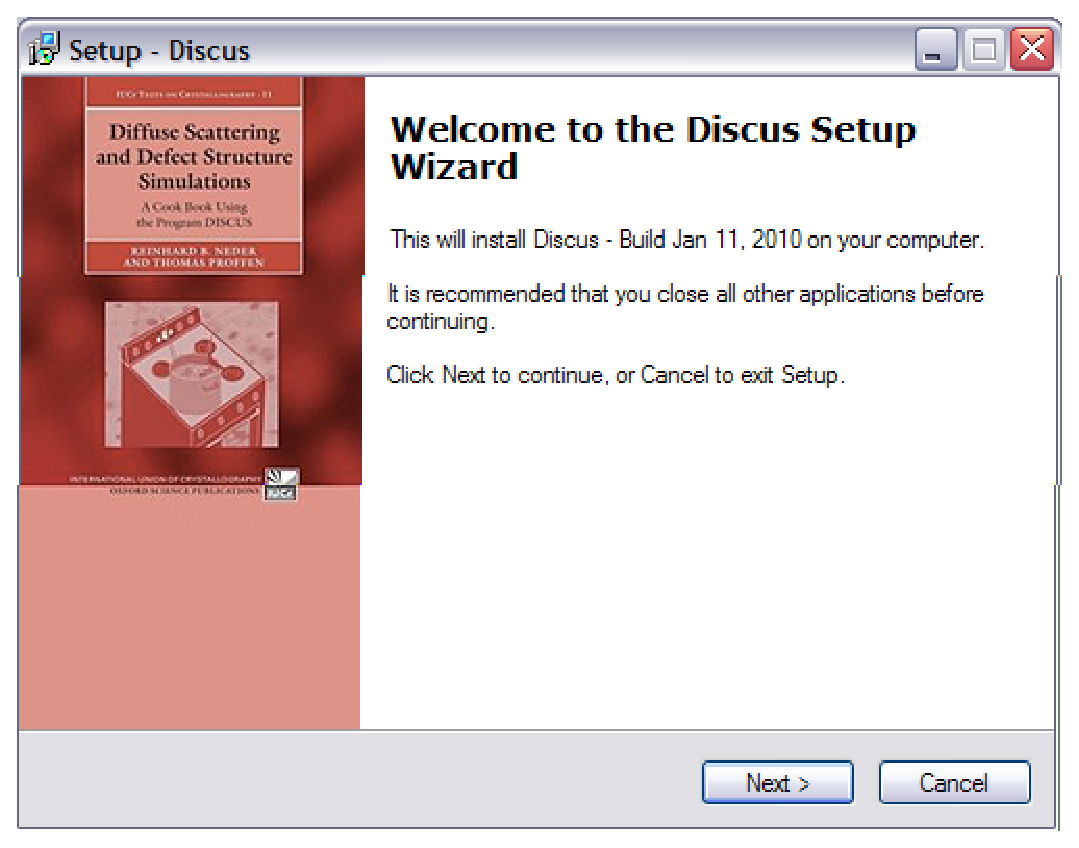
\includegraphics[width=3.0in]{winstall.eps}
%   \hspace{5mm}
%   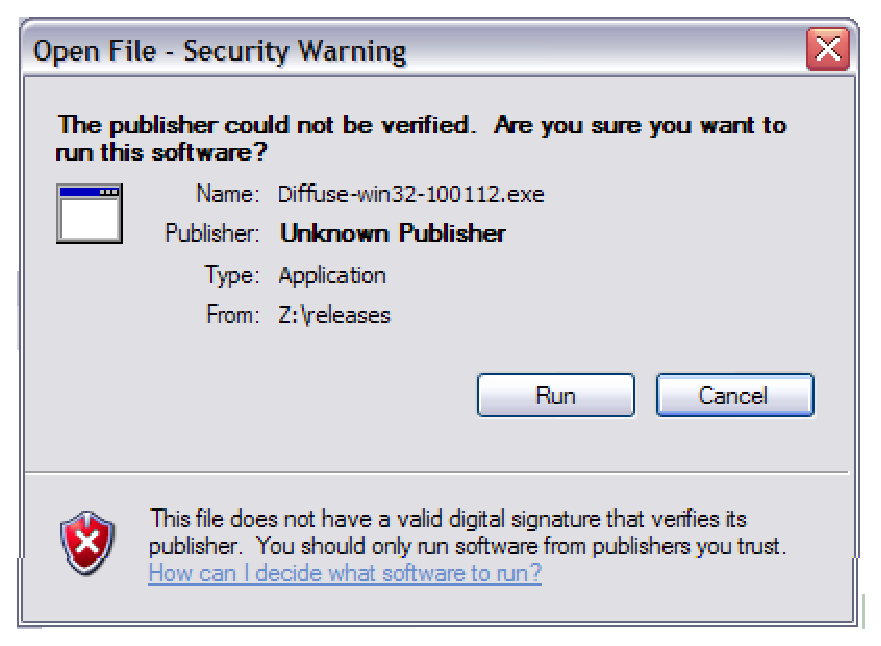
\includegraphics[width=1.7in]{wwarn.eps}
%   \caption{Left: Windows installer for \Discus package.
%            Right: Windows security warning.}
%   \label{fig-winstall}
%\end{figure}

%------------------------------------------------------------------------
\section{Mac OSX\label{appa-bmac}}

The Mac OSX version of the \Discus package is distributed as a binary
installer as well. Simply download the the file {\it Diffuse-mac-YYMMDD.exe}. 
Again YYMMDD specifies the date of the distribution. Make sure you 
download the most recent one. Once the download is finished, run the 
installer by double clicking on the corresponding file icon. You will see 
an installation screen. Follow
%a screen similar to the one shown in Fig. \ref{fig-minstall}. Follow 
the instructions. The programs will be installed in {\tt /Applications/discus}.
%
%\begin{figure}[!tb]
%   \centering
%   \includegraphics[width=3.0in]{minstall.eps}
%   \caption{Mac installer for \Discus package}
%   \label{fig-minstall}
%\end{figure}

%------------------------------------------------------------------------
\section{Unix / Linux \label{appa-bunix}}

For Unix or Linux operating systems, the \Discus package is
distributed as source code and needs to be compiled before the
programs can be used. You might also check the \Discus homepage for
available binary distributions for Linux which might be available
in the near future. 
Refer to the separate file {\tt INSTALL\_DISCUS.pdf} 
or {\tt AAA\_INSTALL\_DISCUS.pdf} for details.

To build the programs from the source, you will 
need a FORTRAN and a C compiler. We use {\tt gcc} and {\tt gfortran}
which are freely available at\\ 
\url{http://directory.fsf.org/project/gcc/}. \\
While {\tt gcc} is installed on most Linux systems, {\tt gfortran} might
need to be installed separately.

First copy or download the file {\it DIFFUSE\_CODE\_YYYY\_MMDD.tar.gz} or
from the github release pages the link to {\it vX.X.X.tar.gz}. Next
unpack the archive using the command

\begin{MacVerbatim}
    tar -xvf DIFFUSE_CODE_YYYY_MMDD.tar.gz
\end{MacVerbatim}

This will create a directory {\it DiffuseCode}, containing the
distribution. Within this directory there are separate directories
for each of the different programs as well as a directory {\it lib\_f90}
which contains command language related routines common to all
programs. Build a a new Directory called {\it DiffuseBuild} next to the
source code directory. Go to this build directory and run ccmake to 
install the program:

Finally some environment variables need to be defined. Each program
looks for a variable corresponding to its name. For example \Discus 
will use a variable {\tt DISCUS} and so on. The definition of 
the variables can be done e.g. in the {\it .login} or {\it .cshrc} file 
using the command {\it setenv DISCUS /path/to/discus} for 
the {\it csh} of {\it set DISCUS=/path/to/discus; export DISCUS} if 
you are using the 
Bourne shell. If this path is also included in your search path you can
start the program simply by entering {\it discus}. Similarly, the
other programs are started by entering their respective names.

%------------------------------------------------------------------------

%\section{Please register}

%Please register yourself as a user of one or more programs of the
%\Discus program package. In the top directory of the
%distribution you will find the file {\tt REGISTER}. Please fill in
%the corresponding information and send the file via email to {\it
%tproffen@lanl.gov}. We also recommend that you subscribe to the 
%{\tt discus-announce@lists.sourceforge.net} mailing list to stay
%informed of the release of new versions of the \Discus package. 
%Details can be found on the \Discus homepage at 
%\url{http://discus.sourceforge.net}.

%------------------------------------------------------------------------

\chapter{COMMON commands}
\section{News}
\par
Here you find a list of recent changes, additions, bug corrections 
\subsection*{2018\_September}
\par
Modified the do and if constructions to be valid as well for 
"end do" "end if" and "else if" with arbitrary blanks. 
\subsection*{2018\_July}
\par
Modified the ==$> $ 'fput' and 'fget' commands to take an optional 
    format string 
\par
Modified the ==$> $ 'system' command to be a bit more flexible 
\par
Modified the ==$> $ function "fmodt" to take a file name as well. 
\subsection*{2018\_June}
\par
Revised the reaction to a CTRL-C 
\par
Added a ==$> $ 'set wait $ \{$"on"$| $"off"$\} $ option 
\par
Added a ==$> $ 'set error, ... , "save" option 
\subsection*{2018\_May}
\par
The variables ==$> $ 'variable' were augmented by 1-D and 2-D arrays. 
New commands ==$> $ 'matmul', 'matadd','invmat', 'mattrans', 
'detmat' provide the usual arithmetics 
\subsection*{2018\_Feb}
\par
New read-only ==$> $ variables "PROGRAM", "STATE", "MPI", "MPI\_FIRST" 
were introduced that can be querried to learn in which program 
section and at what state you are. 
\par
As a patch to overcome internal precision, the ==$> $ 'seed' command 
can take an alternative form. 
\subsection*{2018\_Jan}
\par
The logical comparisons may now take the operators: 
$ <$, $ <$=, ==, /=, $> $=, $> $/ 
The classical fortran77 operators are still valid 
\par
New logical functions "isvar" and "isexp" can be used within an 
"if" construction. See help entry ==$> $'function' 
\par
New parameters "reset" and "delete" have been added to the 
==$> $ 'variable' command 
\subsection*{2017\_November}
\par
A 'manual' command has been added that reads the manual files 
\subsection*{2017\_Sep}
\par
Throughout the program the internal calculation of random numbers 
was changed to the FORTRAN 90 intrinsic function. 
\subsection*{2017\_July}
\par
Predefined variables REF\_* are now read/write. See ==$> $ variable 
\par
Introduced new intrinsic character functions: index and length 
See help under functions for details. 
\subsection*{2016\_October}
\par
New system variables have been introduced. They can be used like any 
other user defined variable. System variables are in capital letters. 
\subsection*{2014November}
\par
A new random number "gskew" has been added, which returns a 
Gaussian distributed random number. The underlying distribution 
can be set to be is left or right skewed. 
\section{Options}
{\bf program [-debug] [-remote] [-port=p] [-access=ip] [macro.mac] \par }
{\bf program -macro $ <$macro.mac$> $[ $ <$par1$> $ [ $ <$par2$> $ ...]] \par }
\par
\vspace{3pt}
All programs allow the following command line parameters. The flag 
"-debug" starts the program in debug mode. This is the same as using 
the command "set debug,on". The switch "-remote" starts the program 
in remote control mode. In this case the commands are send to the 
program through a socket. In this case the switch "-port' allows one 
to specify the port, the program will be listening on. Port numbers 
should be larger than 1024. The switch "-access' allows one to specify 
from which host connections will be accepted. The default is 
'localhost'. 
\par
See file "remote.f" for an example how to remote control the 
applications from another program. Note that the program will not 
accept input from the keyboard when in remote control mode. 
\par
All other command line arguments are interpreted as macro files 
and will be executed at startup. These macros may not rely on 
parameters to be given on the command line. 
\par
If a macro is to be executed that takes 1 or more parameters, use 
the "-macro" option. Note that this option is mutually exclusive 
to all other options. The first command line argument after  the 
'-macro' option it the macro name, all further optional command 
line arguments are taken as macro parameters. These have to be 
seperated by one or more spaces. 
Parameters that need to contain spaces must be enclosed in single 
or double quotation marks. 
-macro test.mac 1 2 3 
This is the same as @test.mac 1,2,3 
\par
-macro test1.mac '1 + 2 + 3' 
This is the same as @test1.mac 1 + 2 + 3 
\section{\#}
{\bf \#$ <$comment$> $ \par }
\par
\vspace{3pt}
Any line beginning with a "\#" is regarded as comment. 
\section{@}
{\bf @$ <$filename$> $ [$ <$argument$> $ ...] \par }
\par
\vspace{3pt}
Any list of valid commands can be written to an ASCII file and 
and indirectly by the command: 
\par
\begin{MacVerbatim}
prompt > @<name>
\end{MacVerbatim}
The commands may start in with leading blanks to help readability of 
the macro file. The commands are executed as typed. 
Macro files may call other macro files. This is not a call in 
the sense of calling a function. 
All variables are identical at all levels of macro file nesting. 
\par
Macro files can be written by any editor on your 
system or be generated by the ==$> $ 'learn' command. 'learn' starts to 
remember all the commands that follow and saves them into the file 
given on the 'learn' command. The learn sequence is terminated by 
the 'lend' command. The default extension is ".mac" 
\par
Optionally arguments can be listed on the command line. These arguments 
will replace the formal parameters inside the macro. The formal 
parameters must be given as "\$1", "\$2" ... The string $ <$argument$> $ will 
replace the string "\$1". "\$1" is the first argument on the command line, 
"\$2" the second and so on. If there are not enough command line arguments, 
an error message is displayed. 
The parameter "\$0" contains the number of parameters listed on the line 
that called the macro. If no parameters were given this value will be 
zero. 
\par
The prompt setting ==$> $ 'set prompt,"redirect"' has an important side 
effect on macro treatment. 
With the "redirect" setting, macros are stored internally, 
once they have been read from disk, and will be reused from memory. This 
helps to reduce unnecessary I/O, especially when you have nested macros 
inside loops. As a side effect, if a macro is modified on the disk, 
a further "@macro.mac" will not read the modified version but will 
continue to use the internaly stored version. 
\par
For all other settings, the internal macro storage is 
cleared when you get back to the normal interactive mode. This allows 
you to run a macro, then modify the version stored on the disk and 
execute the modified/corrected version. 
\section{=}
{\bf $ <$variable$> $ = $ <$expression$> $ \par }
\par
\vspace{3pt}
The expression on the right of the equal sign is evaluated and its result 
stored in variable $ <$variable$> $. 
\section{input}
{\bf Input editing functions \par }
\par
\vspace{3pt}
If the program was compiled with -DREADLINE, the following basic 
editing functions are available at the program prompt: 
\par
\begin{MacVerbatim}
  ^A               : moves to the beginning of the line
  ^B               : moves back a single character
  ^E               : moves to the end of the line
  ^F               : moves forward a single character
  ^K               : kills from current position to the end of line
  ^P or arrow up   : moves back through history
  ^N or arrow down : moves forward through history
  ^H and DEL       : delete the previous character
  ^D               : deletes the current character
  ^L/^R            : redraw line in case it gets trashed
  ^U               : kills the entire line
  ^W               : kills last word
\end{MacVerbatim}
Furthermore you can move within the line using the arrow keys. 
\par
{\bf NOTE: \par }
\par
\vspace{3pt}
If you redirect the input for executed PROG using 'prog $ <$ infile' you 
MUST use the command 'set prompt,off' or 'set prompt,redirect' in 
the first line to avoid that the program 'hangs' at the end of the 
file. (-$> $ set prompt) 
\section{break}
{\bf break $ <$levels$> $ \par }
\par
\vspace{3pt}
The 'break' command stops the execution of the current block structure 
and advances to the next command following the block structure. 
With $ <$levels$> $ equal to 1 only the current block structure is interrupted, 
with any higher number the $ <$levels$> $ innermost block structures are 
interrupted. The 'break' command can be used only inside a block structure. 
\section{cd}
{\bf cd [$ <$directory$> $] \par }
\par
\vspace{3pt}
This command allows one to change the current working directory 
(may not be available everywhere). If the command is called with 
no parameters, the current working directory is shown. 
\par
For the Windows versions, two different styles help to copy the 
folder name into the program window. 
\par
For KUPLOT and the DISCUS\_SUITE type 
cd 
and a space. Do not hit the enter/return key at this moment. 
Within a Windos Explorer click on the folder icon and copy the 
string CTRL-c. Activate the KUPLOT or DISCUS\_SUITE program and 
click the middle mouse button. This should paste the full path 
to the folder into the KUPLOT or DISCUS\_SUITE window. 
\par
For DISCUS, DIFFEV, and MIXSCAT type "cd " with the space as well. 
Now left click and drag the selected folder icon into the program 
window. This should copy the full pathinto the program window. 
Activate the window and hit the ENTER key. 
\section{continue}
{\bf continue [ "prog" ] \par }
\par
\vspace{3pt}
This command is effective only while PROG is in the interrupted 
macro mode or inside interrupted do-loop or if-statements, which serves 
as a debug mode for lengthy macros or block structures 
Make sure you have returned to the same sub menu before you continue! 
\par
Without parameters PROG resumes the execution of a macro or block 
structure in the line following the 'stop' command. If you 
had started another macro while debugging a macro, and this new macro 
contained a 'stop' command as well, the 'continue' command will run 
the remaining lines in the new macro and then stop again at the position 
of the 'stop' command in the outer macro. 
\par
By providing the 'prog' parameter, PROG immediately interrupts all 
macros and returns to the normal prompt. 
If you are in one of the sub sections "discus", "diffev", "kuplot", 
you can continue either with this subsection or go back to the main 
suite if you enter the program name as "suite". 
\section{do}
Loops can be programmed with the 'do' command. The command may take 
the  following forms: 
\begin{MacVerbatim}
do <variable> = <start>,<end> [,<increment>]
  <commands to be repeated>
enddo
\end{MacVerbatim}
Here loops may contain constants or arithmetic expressions 
for $ <$start$> $, $ <$end$> $, and $ <$increment$> $. The internal type of the 
variables is real. The loop counter is evaluated from 
($ <$end$> $ - $ <$start$> $) / $ <$increment$> $ =1 . If this is negative, the loop 
is not executed at all. 
\par
\begin{MacVerbatim}
do while (<logical expression>)
  <commands to be repeated>
enddo
\end{MacVerbatim}
These loops are executed while $ <$logical expression$> $ is true. 
Thus, they may not be executed at all. 
\begin{MacVerbatim}
do
  <commands to be repeated>
enddo until (<logical expression>)
\end{MacVerbatim}
These loops, however, are always executed once, and repeated 
until $ <$logical expression$> $ is true. 
If an error occurs during execution of the loop, the loop is 
interrupted. 
\par
As of version 5.25.1 and later, the word "enddo" 
may also be spelled "end do", where the number of blanks 
that follow the "end" is not significant. 
\section{echo}
\begin{MacVerbatim}
echo [<string>]
echo ["string%dstring",<integer expression>]
echo ["string%Dstring",<integer expression>]
echo ["string%fstring",<float expression>]
echo ["string%Fstring",<float expression>]
echo ["string%cstring",<character expression>]
\end{MacVerbatim}
The string $ <$string$> $ is echoed to the default output device as typed. 
This command serves as a marker inside long macro files. It gives the 
user a chance to include easy to find messages in order to follow 
lengthy or nested structures. 
\par
The alternative command format allows to echo formatted strings to the 
screen. Each "\%d" is replaced by the value of the corresponding 
parameter. The sequence of "\%d" corresponds to the sequence of the 
integer parameters, "\%f" stands for parameters of the type real. 
\par
The value of a numerical expression between the "\%" and the "d" 
determines the width of the integer field that is printed. 
In the case of a floating variable two expressions separated by 
a decimal point specify the width and the number of decimal 
digits that are printed. 
\par
The capital forms "\%D" and "\%F" will fill leading spaces with zeros. 
\par
A character format descriptor "\%c" or "\%Nc", with N an integer 
number, describes a string of characters. 
\par
\begin{MacVerbatim}
Examples
echo ">%3d<",44            produces :  > 44<
echo ">%1+2d<",44          produces :  > 44<
echo ">%3D<",44            produces :  >044<
echo ">%5.1f<",44.1        produces :  > 44.1<
echo ">%2**2+1.1f<",44.1   produces :  > 44.1<
echo ">%c<",'bla'          produces :  >bla<
echo ">%5c<",'bla'         produces :  >bla  <
\end{MacVerbatim}
\section{eval}
{\bf eval $ <$expr$> $ [, $ <$expr$> $ ...] \par }
\par
\vspace{3pt}
Evaluates the expression(s) and displays the result(s). The result is not 
stored, this command is for interactive display only. 
\section{exit}
{\bf exit \par }
\par
\vspace{3pt}
Terminates the program and gets you back to your shell. 
\section{expressions}
\par
Arithmetic expressions can be evaluated in a FORTRAN style. 
Character expressions are used to assign a string of characters to 
a variable or filename. 
\par
\subsection*{Arithmetic expressions:}
\par
Five basic operators are defined: 
\par
\begin{MacVerbatim}
"+"  Addition
"-"  Subtraction
"*"  Multiplication
"/"  Division
"**" Exponentiation
\end{MacVerbatim}
The usual hierarchy of operators holds. 
The parts of the expression can be grouped with parentheses "(",")" in 
order to circumvent the standard hierarchy 
Several intrinsic functions have been defined, see "functions" for a 
full listing. 
\par
Examples of valid expressions are: 
\par
\begin{MacVerbatim}
1
1+3*(sin(3.14*r[1]))
x[1]*0.155
asind(0.5)
\end{MacVerbatim}
\subsection*{Character expressions}
\par
A character expression is signaled by a pair of " ". The content may 
be a just a simple string of characters or additional format 
specifiers that are replaced by the value of a variable. 
\par
\begin{MacVerbatim}
variable character,string
variable character,line
string = "abcdefgh"
line   = "%4c",string(2:5)
line   = "%c %c",string(1:2),string(7:8)
line   = "Number: %3d",4
line   = "Number: %3.1f",4.1
line   = string          ! Both commands work,
line   = "%c",string     ! this is the prefered style
line   = "%c",fdate(0)   ! See ==> functions for a list of
\end{MacVerbatim}
                         ! character functions 
Within an ==$> $ 'if' construction you may also specify a character 
expression in the form: 
\par
\begin{MacVerbatim}
if( '"%2c",string(3:4)' .eq. 'cd' ) then
\end{MacVerbatim}
An expression (M:N) refers to the substring from the M's to the N's 
character. 
\par
\subsection*{Format specifiers}
\par
In filenames ==$> $"filename" or character expressions format specifiers 
are used to write the value of numerical or character variables into 
the corresponding string. These format specifiers may be: 
\par
\begin{MacVerbatim}
%d      writes a decimal/integer number, the number of digits
        depends on the numerical value of the number
%D      writes a decimal/integer number, the number of digits
        depends on the numerical value of the number
%3d     writes a decimal/integer number that fills 3 digits
%3D     writes a decimal/integer number that fills 3 digits,
        leading blanks are filled with zeros
        Any width larger than the number of digits required is allowed
%Md     writes a string M digits wide. M may be omitted.
        M may be an integer expression.
        d or D are allowed, D give leading zeros
%f      A floating/real number is written flushed left into a
        character string of 8 digits
%F      A floating/real number is written flushed left into a
        character string of 8 digits
%12.3f  A floating/real number is written flushed right into a
        character string of 12 digits. 3 digits are used for the
        fractional part.
%12.3F  A floating/real number is written flushed right into a
        character string of 12 digits. 3 digits are used for the
        fractional part. Leading blanks are filled by zeros.
%M.Nf   writes a string M digits wide. N may be omitted.
        M and N may be integer expressions.
        f or F are allowed, F give leading zeros
%c      A character string is written, the width depends on the input
        variable
%5c     A character string of 5 characters is written.
\end{MacVerbatim}
Examples 
\par
\begin{MacVerbatim}
variable character,string
variable character,line
string = "abcdefgh"
line   = "%c",string     ==> "abcdefgh"
line   = "%4c",string(1:4)     ==> "abcd"
line   = "Hallo %c",string(2:4)    ==> "Hallo bcd"
line   = "Number %5d",1234         ==> "Number  1234"
line   = "Number %5D",1234         ==> "Number 01234"
line   = "Float  %8.3f",3.1415     ==> "Float     3.141"
line   = "Float  %8.3F",3.1415     ==> "Float  0003.141"
\end{MacVerbatim}
\section{filenames}
Usually, file names are understood as typed, including capital 
letters. Unix operating systems distinguish between upper and lower 
case typing ! 
\par
Additionally (integer) numerical input can be written into the 
filename. The syntax for this is: 
\par
\begin{MacVerbatim}
"string%dstring",<integer expression>
"string%fstring",<real expression>
"string%cstring",<character expression>
\end{MacVerbatim}
The file format MUST be enclosed in quotation marks. The position of 
each integer must be characterized by a "\%d". The sequence of strings 
and "\%d"'s can be mixed at will. The corresponding integer expressions 
must follow after the closing quotation mark. If the command line 
requires further parameters (like "addfile" for example) they must 
be given after the format-parameters. 
The interpretation of the "\%d"'s follows the C syntax. Up to 10 numbers 
can be written into a filename. 
\par
Refer to the help entry "expressions" for further help. 
\par
Examples: 
\begin{MacVerbatim}
1)
i[5]=1
outfile a1.1
outfile "a%d.%d",1,1
outfile "a%d.%d",4-3,i[5]
outfile "a%1.1f",1.1
\end{MacVerbatim}
All the above examples will result in the file name "a1.1". 
\par
\begin{MacVerbatim}
2)
do i[1]=1,11
...
outfile "data%d.calc",i[1]
...
enddo
\end{MacVerbatim}
The output is written to the files "data1.calc" through "data11.calc" 
\section{fclose}
{\bf fclose $ \{$$ <$number$> $$| $"all"$\} $ \par }
\par
\vspace{3pt}
This command closes a file that was opened with 'fopen $ <$number$> $' or 
closes all open files. If this 
command is not used before exiting the program, data might be lost ! 
\section{fend}
{\bf fend $ <$number$> $,$ \{$'continue'$| $'error'$\} $ \par }
\par
\vspace{3pt}
This command determines the reaction to an unexpected end of file 
while reading data from input file $ <$number$> $. 
If the parameter is set to "continue", the program will set the variable 
res[0] to -1 and continue the macro. If you repeat the  ==$> $ 'fget' 
command, the program will again set res[0] to -1 and will not result 
in an error. In order to catch and EOF, you have to evaluate the 
value of res[0] each time the 'fget' command is executed. 
\par
If the parameter is set to "error", the program will stop reading 
data from the input file and terminate the macro with an error 
message. The value of res[0] remains undefined. 
\par
The default condition at program start is "error" 
\section{fexist}
{\bf fexist $ <$file$> $ \par }
\par
\vspace{3pt}
This command checks the existence of the specified file $ <$file$> $. The 
result is written on the screen and returned via the res[] variables. 
If the file exists, res[1] is 1, otherwise it is 0. The variable 
res[0] returns the number of parameters, here 1. 
\section{fformat}
{\bf fformat $ <$nc$> $,$ <$format$> $ \par }
\par
\vspace{3pt}
This command allows one to specify a FORTRAN style format string 
$ <$format$> $ to be used for column $ <$nc$> $. The default is free format, 
which can be selected using the character * as format string. If 
the command is called with no parameters, the current settings are 
displayed on the screen. Note that an unsuitable format might 
result in a conversion error and *** being written to the file ! 
\par
\begin{MacVerbatim}
Example: fform 1,F7.3
\end{MacVerbatim}
\section{fget}
{\bf fget $ <$number$> $,$ <$p1$> $,$ <$p2$> $,.. \par }
{\bf               [, form:'$ <$string$> $'] \par }
\par
\vspace{3pt}
This command allows the user to read data from a file that had been 
opened with 'fopen $ <$number$> $. If no parameters are given, a line is 
read, yet its content is ignored and the line gets skipped. 
Otherwise the read numbers will overwrite the contents of the 
specified variables. 
The values in the input file must be separated by a blank or a comma. 
This means that to read a set of words in "This is a sentence", you 
will have to read this into 4 character variables. 
\par
Note that a 'fget' command that does not run into an unexpected 
end of file sets the value of res[0] to zero! 
\par
The optional format string allows to specify an input format. 
The format string has to specify the format for each input parameter. 
It thus takes a comma delimited list of Fortran style descriptors: 
i$ <$length$> $         Integer = Whole number 
                  As in "i4"  or "i17" 
f$ <$length$> $.$ <$dec$> $   Floating point number: 
                  As in "f8.3". Only the overall length $ <$length$> $ 
                                is relevant, the length of the 
                                digits after a decimal point is ignored. 
                                Thus, other than in Fortran you 
                                can write: 
f$ <$length$> $         As in "f8" or "f12" 
a$ <$length$> $         Character = alphanumeric string 
                  As in "a20" 
\par
Example: 
Assume a file "example.text" with the following content: 
\par
3.1415  123456 
2.7182817 Hello 654321 
This is a sentence 
\par
This can be read with the following instructions 
\par
fopen 1, example.text 
variable character, str\_a 
variable character, str\_b ! formats are optional for line 1, and 2 
fget 1, r[2],i[2]         , form:'f6,i8' 
fget 1, r[2],str\_a,i[2]   , form:'f9.7,a5,i7' 
fget 1, str\_b             , form:'a18'        ! whole string is read 
fclose 1 
\section{fopen}
{\bf fopen $ <$number$> $,$ <$file$> $ [,$ \{$"append" $| $ "overwrite"$\} $] \par }
\par
\vspace{3pt}
This command allows the user to open a file for reading and writing 
using the commands 'fget' and 'fput'. The first argument is the number 
of the io\_stream. You can open several files at once, the exact value 
depends on the value of the variable MAC\_MAX\_IO in file "macro.inc". 
The second argument is the file name. The default is that existing 
files will be overwritten if 'fput' is used. Alternatively one can 
append data to a file by specifying the optional parameter "append". 
\section{fput}
{\bf fput $ <$number$> $,$ <$p1$> $,$ <$p2$> $, .. \par }
{\bf               [, form:'$ <$string$> $'] \par }
\par
\vspace{3pt}
This command allows one to write data to the file that had been opened 
by 'fopen $ <$number$> $'. The parameters $ <$pi$> $ can either be variables and 
expressions or simple text enclosed in single quotes. If no parameters 
are given, an empty line is written. 
In order to mix character variables or character functions and numbers, 
the first parameter must be a format descriptor in double "". 
\par
The optional format string allows to specify an output format. 
The format string has to specify the format for each input parameter. 
It thus takes a comma delimited list of Fortran style descriptors: 
i$ <$length$> $         Integer = Whole number 
                  As in "i4"  or "i17" 
f$ <$length$> $.$ <$dec$> $   Floating point number: 
                  As in "f8.3". Total width is 8 digits with 3 
                                digits after a decimal point. 
a$ <$length$> $         Character = alphanumeric string 
                  As in "a20" 
\par
The optional format string effectively replaces the 
==$> $ 'fformat' command. 
\par
\begin{MacVerbatim}
Examples:  fput 1, i[1],sqrt(1.0+i[1]*0.01)
           fput 1, 'Current value of i[1] : ',i[1]
           fput 1, "%c %d",'Current value of i[1] : ',i[1]
           fput 1, "%c",fdate(0)
           fput 1, 1,2,3, form:'i3,i3,i3'
           fput 1, 1,3.1415,3, form:'i3,f8.4,i3'
\end{MacVerbatim}
\section{fsub}
{\bf fsub $ <$number$> $,[$ <$left$> $,$ <$right$> $] \par }
\par
\vspace{3pt}
The command allows you to limit the string from which 'fget' reads the 
data from file $ <$number$> $. Data will only be read columns $ <$left$> $ to $ <$right$> $. 
If both parameters are missing, the full input string is read. 
If the parameter $ <$right$> $ is set to "-1", the string is read from $ <$left$> $ 
all the way to the end of the input string, independent of its length. 
\par
The default values at program start are 1,-1 for all input channels. 
\par
\begin{MacVerbatim}
Examples:
  Input line: "A text string 20.0  30.0"
  fsub 14,24
  fget r[1],r[2]
\end{MacVerbatim}
\section{functions}
\par
The following intrinsic numerical functions exist: 
\par
\begin{MacVerbatim}
asin(<arg>)                     !
acos(<arg>)                     !
atan(<arg>)                     !
atan(<arg1>,<arg2>)             ! Arguments are sine and cosine of angle
asind(<arg>)                    ! Result in degrees
acosd(<arg>)                    ! Result in degrees
atand(<arg>)                    ! Result in degrees
atand(<arg1>,<arg2>)            ! Arguments are sine and cosine of angle
sin(<arg>)                      !
cos(<arg>)                      !
tan(<arg>)                      !
sind(<arg>)                     ! Argument in degrees
cosd(<arg>)                     ! Argument in degrees
tand(<arg>)                     ! Argument in degrees
sinh(<arg>)                     ! Hyperbolic functions
cosh(<arg>)                     !
tanh(<arg>)                     !
sqrt(<arg>)                     ! Square root of <arg>
exp(<arg>)                      ! exponential (base e)
ln(<arg>)                       ! natural logarithm of <arg>
abs(<arg>)                      ! Absolute value of <arg>
mod(<arg1>,<arg2>)              ! Modulo <arg1> of <arg2>, real arguments
max(<arg1>,<arg2>)              ! Maximum of <arg1> and <arg2>
min(<arg1>,<arg2>)              ! Minimum of <arg1> and <arg2>
int(<arg>)                      ! Convert argument to integer
nint(<arg>)                     ! Convert argument to nearest integer
frac(<arg>)                     ! Returns fractional part of <arg>
ran(<arg>)                      ! Returns uniformly distributed pseudo
                                  random value 0<= r < 1.
gran(<arg>{,"s"|"f"})           ! Returns gaussian distributed pseudo
                                  random value with mean 0.0 and
                                  sigma <arg> or FWHM <arg> if the
                                  second argument is equal to "f".
gskew(<arg>,<skew>{,"s"|"f"})   ! Returns gaussian distributed pseudo
                                  random value with mean 0.0 and
                                  sigma <arg> or FWHM <arg> if the
                                  second argument is equal to "f".
                                  If skew is 0 the distribution is symmetric
                                  For skew <=  1.0 it is right skewed
                                  For skew >= -1.0 it is left  skewed
logn(<arg1>,<arg2>{,"s"|"f"})   ! Returns lognormal distributed pseudo
                                  random value. <arg1> is the location
                                  of the most likely value.
                                  <arg2> is the width of the distribution.
                                  More accurately, <arg2> is the width of
                                  the underlying distribution ln(logn).
                                  It is either sigma <arg2> or FWHM <arg2>
                                  if the third argument is equal to "f".
pois(<arg>)                     ! Returns Poisson  distributed pseudo
                                  random value with mean <arg>.
\end{MacVerbatim}
The arguments to any of these functions are any arithmetic expression. 
\par
System functions: 
\par
\begin{MacVerbatim}
date(0)                         ! Returns the current date as character
                                  string in the format:
                                  CCYYMMDDhhmmss.sss
                                  CCYY  : year    (century, year)
                                  MM    : month   (1,2,... 12)
                                  DD    : day     (1,2,... 31)
                                  hh    : hour    (1,2,... 24)
                                  mm    : minute  (1,2,... 60)
                                  ss.sss: second.milliseconds
                                  (g77: milliseconds are 000)
fdate(0)                        ! Returns the current date as character
                                  string in the format:
                                  Day Mon DD hh:mm:ss CCYY
                                  Day   : weekday (Mon, Tue,... Sun)
                                  Mon   : month   (Jan, Mar,... Dec)
                                  DD    : day     (1,2,... 31)
                                  hh    : hour    (1,2,... 24)
                                  mm    : minute  (1,2,... 60)
                                  ss    : second  (1,2,... 60)
                                  CCYY  : year    (century, year)
fmodt(0)                        ! Returns modification date and time
                                ! of the last file that was opened by
                                ! the Discus_suite.
fmodt('name')                   ! Date for file "name"
fmodt(<line>)                   ! Date for file in variable <line>
                                ! The format ! is the same as for fdate(0)
getcwd(0)                       ! Returns the current directory as
                                  character string.
getenv('name')                  ! Returns the value of the environment
                                  variable "name".
getenv(<line>)                  ! Returns the value of the environment
                                  variable that is stored in variable <line>.
index(<line>, <substring> [,"BACK"]) ! Returns the location of the
                                  substring within the line.
                                  If the optional keyword "BACK" is present,
                                  index returns the last occurence.
                                  Both, the line and the substrings may be
                                  given as simple strings in single quotations
                                  or as a variable with with a preceeding
                                  format specifier, Examples:
                                  line ='Discus'
                                  index('Discus','s')
                                  index('Discus','s', BACK)
                                  index("%",'Discus',"%",'s')
                                  index("%",line    ,"%",'s')
                                  index("%c",getcwd(0), '/')
length(<line>)                    !Returns the length of string <line>
                                  The line may be
                                  given as simple strings in single quotations
                                  or as a variable with with a preceeding
                                  format specifier, Examples:
                                  length('Discus')
                                  length("%c",line)
                                  index("%c",getcwd(0), '/')
isvar('string')                   Returns TRUE if the string is a used
                                  defined variable. Can only be used inside
                                  an if construction:
                                  Examples:
                                  if(isvar('name')) then
                                  if(isvar('$1')) then
isexp('string')                   Returns TRUE if the string is a valid
                                  expression. Can only be used inside
                                  an if construction:
                                  Examples:
                                  if(isexp('3+5.')) then
                                  if(isexp('$1')) then
\end{MacVerbatim}
\section{help}
{\bf help [$ <$command$> $ [, $ <$subcommand$> $] ] \par }
\par
\vspace{3pt}
The 'help' command is used to display on-line help messages. They are 
short notes on the command $ <$command$> $. The command may be abbreviated. 
If the abbreviation is not unique, only the first help topic that matches 
the command is listed. 
\par
The first line of the help text gives the syntax of the command that is 
explained in the following lines. For a few commands the syntax line is 
repeated for different set of possible parameters. 
\par
After the text is displayed, you are in the HELP sublevel of PROG 
and there are the following commands possible: 
\par
\begin{MacVerbatim}
<command> : Display help for <command> of current help level.
".."      : Go up one help level.
"?"       : Prints list of help entries of the current level.
<RETURN>  : Exit help sublevel.
\end{MacVerbatim}
\section{if}
The if-control structure takes the following form: 
\par
\begin{MacVerbatim}
if ( <logical expression> ) then
  <conditional commands>
[elseif ( <logical expression>) then
  <conditional commands>]
[else
  <conditional commands>]
endif
\end{MacVerbatim}
The logical expressions may contain numerical comparisons with syntax: 
\par
As of version 5.25.1 and later, the words "elseif" and "endif" 
may also be spelled "else if" or "end if", where the number of blanks 
that follow the "end" is not significant. 
\par
\begin{MacVerbatim}
<arithmetic expression> <operator> <arithmetic comparison>
\end{MacVerbatim}
The following operators are allowed: 
\par
\begin{MacVerbatim}
 <      ! less than
 <=     ! less or equal
 >      ! greater than
 >=     ! greater or equal
 ==     ! equal
 /=     ! not equal
\end{MacVerbatim}
The older forms are still valid: 
\begin{MacVerbatim}
.lt.    ! less than
.le.    ! less or equal
.gt.    ! greater than
.ge.    ! greater or equal
.eq.    ! equal
.ne.    ! not equal
\end{MacVerbatim}
The logical expressions may also contain string comparisons with syntax: 
\par
\begin{MacVerbatim}
'<string1>' <operator> '<string2>'
\end{MacVerbatim}
Both strings MUST be enclosed by single apostrophes '. The operators 
are the same as those for the numeric expressions, lexical comparisons 
are used to evaluate the comparisons "less" and "greater". 
Within the single apostrophes you can place a character replacement 
operation. Thus a valid example would be: 
variable character, line 
line='text' 
if( '"\%c",line' .eq. 'text' ) then 
\par
Logical expressions can be combined by logical operators: 
\par
\begin{MacVerbatim}
.not.   ! negation of the following expression
.and.   ! logical and
.eqv.   ! logical equivalent
.xor.   ! logical exclusive or
.or.    ! logical or
\end{MacVerbatim}
Logical operations may be nested and grouped by brackets "(" and ")". 
\section{learn}
{\bf learn [$ <$name$> $] \par }
\par
\vspace{3pt}
Starts a learn sequence. All following commands are saved as typed 
in file $ <$name$> $. defaults to "$ <$prog$> $.mac". ==$> $ lend finishes the 
learn sequence. 
\section{lend}
{\bf lend \par }
\par
\vspace{3pt}
Finishes the learn sequence started by ==$> $ learn. 
\section{manual}
{\bf manual ["section:"$ \{$"suite"  $| $ "discus"  $| $ "diffev" $| $ \par }
{\bf                    "kuplot" $| $ "package" $| $ "mixscat"$\} $ \par }
{\bf        [,"viewer:"$ <$name$> $] \par }
\par
\vspace{3pt}
Opens a PDF viewer for one of the Manuals 
\par
The section defaults to the current program section that you are 
working with. 
On Linux systems, the viewer defaults to "qpdfview", on Windows 
system it defaults to "firefox". If DISCUS does not find the 
default or the user provided viewer, DISCUS will search 
a list of common PDF viewers. If none is found an error message 
points to the folder that contains the manuals. 
\section{seed}
{\bf seed [ $ <$value$> $ ] \par }
{\bf seed [ $ <$value\_a$> $, $ <$value\_b$> $ ] , group:$ <$no$> $ \par }
\par
\vspace{3pt}
Reinitializes the pseudo random generator. The seed passed to the 
random generator is -abs(nint(value)). If the $ <$value$> $ is omitted, 
the random generator will be passed the number of hundredth of 
seconds passed since midnight, essentially initializing the sequence 
at a unknown fairly random point. 
\par
The seed may take more than one parameter, usually the compiler 
takes 12 different seeds. 
\par
To overcome limited internal precision, a patch has been introduced 
in version 5.17.0. 
As the random number generator takes seeds in the range from 
1 to 99999999 the internal precision that calculates the value 
on the command line via the detour of a real valued number turned 
out to be insufficient. To ensure that an eight digit seed number 
is properly transfered to the seed initialization routine, split 
the number into two groups of four digit integers as in: 
12345678  =$> $ 1234, 5678, group:2 
The optional parameter "group" tells the SUITE to group these two 
numbers together to the original intended eith digit no. 
\section{matrix}
\par
For the user defined 1-D and 2-D matrices several command are 
available for the usual matrix arithmetics. These are: 
\subsection*{detmat}
{\bf detmat $ <$matrix$> $ \par }
\par
\vspace{3pt}
Calculates the determinant of a [n x n] matrix. Currently limited 
to dimensions 1 to 4. 
\subsection*{invmat}
{\bf invmat $ <$result$> $, $ <$input$> $ \par }
\par
\vspace{3pt}
Calculates the inverse matrix for $ <$input$> $ and stores the result 
in $ <$result$> $. Both matrices must be square with identical 
dimenstions 1 to 4. 
\subsection*{matmul}
{\bf matmul $ <$result$> $, $ <$a$> $ [, $ <$b$> $] \par }
\par
\vspace{3pt}
A generic name for several calculations. Mainly, of course, the 
standard matrix multiplications of user defined variables 
$ <$a$> $ with $ <$b$> $. 
Either or both of $ <$a$> $ and $ <$b$> $ may be arbitrary scalar expressions. 
The result and the input matrices may be 1-D and or 2-D 
according toi the standard rules for matrix multiplications 
\par
Thus the command essentially provides the operations: 
\par
1) Result\_matrix = Scalar 
2) Result\_matrix = Scalar * Scalar 
3) Result\_matrix = Scalar * Matrix = Matrix * Scalar 
4) Result\_matrix = Matrix 
5) Result\_matrix = Matrix * Matrix 
\par
1) and 2): Each matrix element is set to the scalar value 
    Result[i,j] = scalar 
3): Each input matrix element is multiplied by the scalar 
    and each result element corresponds to the input matrix 
    element 
    Result[i,j] = scalar * Input[i,j] 
4): The result matrix is identicla to the input matrix 
    Result[i,j] = Input[i,j] 
5): Standard matrix multiplication 
    Result[i,j] = A[i,k] * B[k,j] 
\par
For operations 3 and 4, both matrices must be of identical 
shape and dimension. 
For operation 5 the standard rule on shape and dimensions 
holds with 
    Result[i,j] = A[i,k] * B[k,j] 
\subsection*{matadd}
{\bf matadd $ <$result$> $, $ <$a$> $ [, $ <$scalar$> $], $ <$b$> $ \par }
\par
\vspace{3pt}
Adds two user supplied matrix variables. 
    Result[i,j] = A[i,j] + Scalar * B[i,j] 
\par
The three matrices have to be of identical shape and dimensions, 
The scalar is optional and defaults to +1. 
The result matrix may be the same variable as any of the 
two input matrices. 
\subsection*{mattrans}
{\bf mattrans $ <$resul$ <$, $ <$input$> $ \par }
\par
\vspace{3pt}
Calculates the transposed matrix for $ <$input$> $ and stores this 
in $ <$result$> $ 
\par
\section{set}
{\bf set $ <$command$> $,.. \par }
\par
\vspace{3pt}
This command allows to alter various program independent setting. 
Allowed values for $ <$command$> $ are: 
\par
\subsection*{prompt}
{\bf set prompt, $ \{$"on"$| $"off"$| $"redirect"$\} $,[$ \{$"on"$| $"off"$| $"file"$\} $, ["save"]] \par }
{\bf set prompt, "old" \par }
\par
\vspace{3pt}
First parameter sets the status of the PROG prompt. The default is 
"on", i.e. PROG prompts for the next command by writing "discus $> $ " 
(in case you run DISCUS ..). You can turn this prompt off. This is 
useful, if you are running a long macro and do not 
want to get all the prompts written into the output. By using this 
option you can considerably shorten the output written by PROG into a 
redirected log file. If you are using PROG on a UNIX platform, you can 
start the program with redirected input by the command: 
\par
\begin{MacVerbatim}
"prog < inputfile"
\end{MacVerbatim}
By default, PROG will write the prompt "discus $> $" into the output file, 
expecting a RETURN from the keyboard. Very long lines in the output file 
will result. To avoid this situation insert the line "set output,redirect" 
as first line in the inputfile to force discus to echo the lines from file 
inputfile. 
\par
The prompt setting "redirect" has an important side effect on macro 
treatment. With the "redirect" setting, macros are stored internally, 
once they have been read from disk, and will be reused from memory. This 
helps to reduce unnecessary I/O, especially when you have nested macros 
inside loops. For all other settings, the internal macro storage is 
cleared when you get back to the normal interactive mode. This allows 
you to run a macro, then modify the version stored on the disk and 
execute the modified/corrected version. 
\par
This second parameter  allows the user to assign where the text output 
of the program should go: "on" prints on the screen, "off" will result 
in no output and "file" will save the output to a file progname.log 
(e.g. discus.log in DISCUS). Note that the output of the commands 
'echo' and 'eval' will always appear on the screen. The last parameter 
allows on to save the current prompt and output settings. 
\par
The parameter "old" allows the user to restore the setting of the 
prompt and output. This can e.g. be used to turn the prompt off in a 
macro and then restore the original setting after the macro is executed. 
Make sure that you saveed the desired prompt by setting the last 
parameter to "save". 
\subsection*{error}
{\bf set error , $ \{$"cont" $| $ "exit" $| $ "live" $| $ "old"$\} $ [ , "save"] \par }
\par
\vspace{3pt}
Sets the error status. 
\par
\begin{MacVerbatim}
"cont"  PROG returns the normal prompt after the display of the error
        message. You can continue the input of commands.
        The execution of a macro file is stopped, the program continues
        with the regular prompt of the menu/submenu where the error occurred.
"exit"  PROG terminates after the display of the error message.
        This option is useful if you run PROG in the batch mode of your
        operating system. Instead of continuing with a faulty calculation
        PROG stops and you can immediately check the error.
"live"  PROG remains alive after an error is encountered. The variable
        "res[0]" is set to -1. The error number is written into "res[1]",
        the error type to "res[2]". Further error codes are written into
        "res[3]".
        With this error status, the program remains alive within a loop
        as well, which it does not do with the error status "cont".
        The program also continue to execute a macro!
        It is most helpful to catch errors from the 'system' command
        and to allow a flexible response.
"old"   Restore the last error status that was set and saved in a
        previous 'set error, <value>, save ' command.
\end{MacVerbatim}
\subsection*{debug}
{\bf set debug, $ \{$"on" $| $ "off"$\} $ \par }
\par
\vspace{3pt}
This command allows the user to enable various DEBUG outputs ... 
\subsection*{wait}
{\bf set wait, $ \{$"on" $| $ "off"$\} $ \par }
\par
\vspace{3pt}
This command allows the user to tailor the 'wait' comand. 
The default is 'set wait, on'. 
With 'set wait, on' the 'wait' command in a macro is active. 
With 'set wait, off' the 'wait' command in a macro will be 
ignored and the programm continues execution as if the 
'wait' command were absent. 
\section{show}
{\bf show $ \{$"res" $| $ "variables"$\} $ \par }
\par
\vspace{3pt}
The show command displays settings onto your screen. The individual 
programs discus, kuplot, diffev, mixscat all have specific parameters 
to the show command as well, see the help at the main program level 
for details. 
\par
\begin{MacVerbatim}
"res"
\end{MacVerbatim}
Many commands produce results that are stored in the result variable 
res[$ <$i$> $]. Thise are displayed via "show res". 
The entry res[0] gives the number of entries in the result variable. 
\par
\begin{MacVerbatim}
"variables"
\end{MacVerbatim}
Lists the variables that have been defined, their type and their 
current values. The command is identical to the "variable show" 
command. 
\section{sleep}
{\bf sleep $ <$seconds$> $ \par }
\par
\vspace{3pt}
This command causes the program to sleep for $ <$seconds$> $ seconds 
\section{socket}
{\bf socket "open",$ <$host$> $,$ <$port$> $ \par }
{\bf socket "close" \par }
{\bf socket "exit" \par }
{\bf socket "send",$ <$string$> $ \par }
{\bf socket $ <$string$> $ \par }
{\bf socket "transfer",$ <$slave\_var$> $,$ <$expression$> $ \par }
{\bf socket "transfer",$ <$slave\_var$> $,$ <$character expression$> $,$ <$local\_var$> $ \par }
\par
\vspace{3pt}
These commands connect to a program that has been started with the 
"-remote" option, sees ==$> $ "Options" for further help. 
The commands will be send to the slave program where they will be 
executed as typed. 
\par
\subsection*{open}
{\bf socket "open",$ <$host$> $,$ <$port$> $ \par }
\par
\vspace{3pt}
Opens the connection to the program running on host $ <$host$> $ and 
listening on port $ <$port$> $. The server program  must have been 
started beforehand with the "-remote" option 
\subsection*{close}
{\bf socket close \par }
\par
\vspace{3pt}
Temporarily closes the connection to the slave program, which keeps 
running. You can open to the same program with a new socket open,$ <$pname$> $. 
\subsection*{exit}
{\bf socket exit \par }
\par
\vspace{3pt}
Terminates the slave program and closes the connection. To communicate 
with the slave program again, you must first start this with the 
"-remote" option and then open the connection with 
socket "open",$ <$pname$> $. 
\subsection*{send}
{\bf socket send,$ <$string$> $ \par }
{\bf socket $ <$string$> $ \par }
\par
\vspace{3pt}
The string is send to the slave program and executed as typed. 
Both forms are equivalent. 
\subsection*{transfer}
{\bf socket transfer,$ <$slave\_var$> $,$ <$expression$> $ \par }
{\bf socket transfer,$ <$slave\_var$> $,$ <$character expression$> $,$ <$local\_var$> $ \par }
\par
\vspace{3pt}
This command transverse the value of $ <$expression$> $ to the slave 
variable $ <$slave\_var$> $. You must define this slave variable prior 
to a transfer. 
\subsection*{Example}
\par
\begin{MacVerbatim}
system /usr/local/bin/kuplot -remote   ! starts kuplot slave
i[0] = 4.0                             ! set local variable
socket open,localhost,3331             ! open connection
socket func r[0]**2,-2,2,0.1           ! define a function to plot
socket transfer,i[1],i[0]              ! transfer local variable
socket tit1 "%d",i[1]                  ! set plot title
socket plot                            ! display plot
socket mark 1,1                        ! change marker interval
socket plot                            ! plot again
socket send, mark 0.5,0.5              ! change marker interval
socket send, plot                      ! plot again
socket exit                            ! terminate kuplot, exit
\end{MacVerbatim}
\section{stop}
{\bf stop \par }
\par
\vspace{3pt}
This command is active only while reading from a macro file or in 
interactive mode inside a block structure (do-loops and/or if's). 
\par
The current macro file is interrupted and you can type commands as in the 
normal input mode. You can use the whole range of PROG commands, 
including the '@' macro command. The 'stop' commands provides a convenient 
mode to debug a macro by setting a break point at which you can check the 
value of variables or set new values, run an additional macro etc. 
\par
To continue execution of the macro or to continue with the normal 
PROG mode, use the ==$> $ 'continue' command. 
\par
If included in a block structure statement (do-loops and/or if's) in 
both, macro and interactive mode, the program continues reading all 
statements that belong to the block structure. During execution of the 
structure, PROG interrupts this execution if it encounters a 'stop' 
command. You can issue any PROG command except further do or if commands. 
\par
To continue execution of the structure or to continue with the normal 
PROG mode, use the ==$> $ 'continue' command. 
\section{system}
{\bf system $ <$com$> $ \par }
{\bf system "string\%dstring",$ <$integer expression$> $ \par }
{\bf system "string\%fstring",$ <$float expression$> $ \par }
\par
\vspace{3pt}
Executes the single shell command $ <$com$> $. 
If the command string is enclosed in "", you can place integer and 
real format specifiers "\%d" "\%f" which are then substituted by the 
corresponding values. 
The shell command $ <$comm$> $ may be placed in front of the double 
quotation marks. 
\par
Example 
i[0]=10 
system "ls \%d.*" 
system ls "\%d.*" 
\par
This would list all files called 10.* 
\section{wait}
{\bf wait [$ \{$"return" $| $ "input" [,$ <$prompt$> $] $\} $] \par }
\par
\vspace{3pt}
This command waits for user input. 
Without a parameter or with "return", the program waits for a 
simple $ <$RETURN$> $. 
If the first parameter is "input", the program expects the user to enter 
one or more real numbers or expressions. The optional $ <$prompt$> $ can be 
used to ask the user to input the expressions. This is especially 
helpful if the prompt has been turned of by ==$> $ set prompt,off. 
The number of expressions entered by the user is stored in the variable 
res[0] and the results of the expressions in res[i]. 
\par
This command allows to write interactive macros, demo macros 
and tutorials. 
\par
With the command 
{\bf set wait, $ \{$"on" $| $ "off"$\} $ \par }
\vspace{3pt}
you can toggle the active state of the wait command on off. 
\par
The default is 'set wait, on'. 
With 'set wait, on' the 'wait' command in a macro is active. 
With 'set wait, off' the 'wait' command in a macro will be 
ignored and the programm continues execution as if the 
'wait' command were absent. 
\section{variable}
\begin{MacVerbatim}
variable {"integer"|"real"},<name> [,<initial_value>] [,dim:[d1,d2]]
variable {"character"},<name>
variable show
variable reset
variable delete {,"all"| <name>..]
\end{MacVerbatim}
The programs that are part of the DIFFUSE suite offer predefined 
variables i[*] and r[*]. These are an integer and a real 
array, respectively, into whose element you may store appropriate 
values. 
In order to enhance readability of a macro, you can define your 
own variable names by the use of this command. The variable may 
either be an integer or a real variable. There is no predefined 
syntax for the variable names. Optionally you can initialize the 
variable to $ <$initial\_value$> $, default is zero. These user defined 
variables may be used just as the system integer and real 
variables i[*] and r[*]. 
Character variables may be used to hold a string of text. 
\par
The variable names may only consist of alphanumerical characters 
including the underscore "\_". 
"Real" and "Integer" variables my optionally be declared as 
one or two dimensional arrays. Specify the dimension as: 
dim:[12]  for a 1-D array of length 12 
dim:[3,3] for a 2-D array of length 3x3 
Array indices start at 1. 
Presently character variables are single value variables. 
\par
Several system variable exist that are read only. Several of 
these refer to the refinement section DIFFEV. These variables 
all start with "REF\_". See the DIFFEV on-line help and manual 
for further details. 
\par
If the first command parameter is "show" the program displays a 
list of user defined variables and their current values. 
Refer to the help entry "expressions" for further help. 
\par
Both, the "reset" and the "delete, all" parameters specify that 
the variable list is to be cleared of all user defeined variables. 
Only the system variables remain. 
\par
Alternatively, the "delete, $ <$name$> $" parameters allow you to delete 
an individual variable. 
\par
Examples: 
\begin{MacVerbatim}
variable  int,alpha,90
variable  int,beta
variable  real,diff
beta = 94
diff = alpha - beta
eval diff
variable  character,string
variable  character,line
string = "abcdefg"
line   = "%3c",string(2:4)
var show
\end{MacVerbatim}
Variable names that are part of intrinsic functions, keywords like 
"do", "elseif", "eq", and program specific variables like "r" and "i" 
are not allowed. Thus a variable called "a" is illegal, since it 
is part of the intrinsic function "asin". 
\par
Internally the program sorts the variable names by length and in 
inverse alphabetical order. This sorting has no serious consequence 
for the user other than finding the variable in the printed list 
when using the 'variable show' command. 
\par
A few predefined variables exist, their names are capitalized: 
PI  3.1415... 
REF\_GENERATION  Current generation number as set by DIFFEV 
REF\_MEMBER      Current population size   as set by DIFFEV 
REF\_CHILDREN    Current child population size as set by DIFFEV 
REF\_DIMENSION   Current Number of parameters a set by DIFFEV 
                If the value is changed, you can store more 
                values in ref\_para[], but this does NOT change 
                the actual dimension pop\_dimx that DIFFEV uses. 
PROGRAM         Tells you in which section you are possible 
                values are SUITE=0, DISCUS=1, DIFFEV=2, KUPLOT=3 
STATE           Tells you whether this is the TOP=0 level, a 
                SECTION=1 or a BRANCH=2. 
MPI             Was the program started with MPI ? 
                MPI\_ON=1, MPI\_OFF=0 
MPI\_FIRST       Is this the first call to DIFFEVs ==$> $ 'run\_mpi' 
                command with the current GENERATION? FALSE=0 TRUE=1 
\section{errors}
\par
The program has been written such that it should handle almost 
any typing error when giving commands and hopefully all errors 
that result from calculation with erroneous data. When an error 
is found an error message is displayed that should get you back 
on track. See the manual for a complete list of error messages. 
In this part we refer to the program you are using as DISCUS for 
convenience. 
\par
The error messages concerning the use of the command language 
are grouped in the following categories: 
\par
\begin{MacVerbatim}
COMM   Command language errors
FORT   Fortran interpreter errors
I/O    Errors regarding input/output
MACR   Errors related to macros
MATH   General mathematical errors
\end{MacVerbatim}
Each error message is displayed together with the corresponding 
category $ <$cccc$> $ and the error number $ <$numb$> $ in the form: 
\par
\begin{MacVerbatim}
****CCCC****message                    **** numb ****
\end{MacVerbatim}
In the default mode DISCUS returns the standard prompt and you can 
continue the execution from this point. You can set the error status 
to "exit" by the ==$> $'set' command. In this case DISCUS terminates 
if an error is detected. This option is useful to terminate a faulty 
sequence of commands when running DISCUS in the batch mode of your 
operating system. 
\par
\subsection*{comm}
\par
Command language errors 
These messages describe illegal usage of the command language, such as 
unknown commands, improper numbers of parameters. 
\par
\subsubsection{Error -1: DISCUS directory not defined}
\par
The environment variable DISCUS\_DIR was not defined. Check the chapter 
on installation for your platform for the appropriate definition. 
\subsubsection{Error -2: Command parameter has zero length}
\par
On the command line you probably have a typing error like two 
comma following each other without significant values in between, 
or the first non blank character after the command is a comma. 
\subsubsection{Error -3: Could not allocate arrays}
\par
The program has to allocate arrays, but received a error message. 
Does your computer have enough available memory space? 
\subsubsection{Error -5: Error in operating system command}
\par
The operating system/shell returned an error message. Check the 
appropriate system manuals for details. 
\subsubsection{Error -6: Missing or wrong parameters for command}
\par
Either the command needs more parameters than were provided, or the 
parameters are incorrect. Check the number and type of parameters. Is 
the sequence of numerical and character parameters correct? 
\subsubsection{Error -8: Unknown command}
\par
The command interpreter read an unknown command. Check the spelling 
of the command or check, whether this command is allowed at the current 
sublevel. 
\subsubsection{Error -11: Error in subroutine}
\par
More or less a system error message, ignore this message. 
\subsubsection{Error -17: Too many parameters}
\par
More parameters have been provided than are required by the command. 
Check the number, and type of parameters supplied, or the occurrence 
of additional ','. 
\subsection*{fort}
\par
Fortran interpreter errors 
These messages describe erroneous mathematical calculations and 
improper usage of control structures (do,if, ...). 
\par
\subsubsection{Error -1: Nonnumerical Parameters in expression}
\par
The interpreter found a nonnumerical string where a number is expected. 
If an intrinsic function or a variable was intended, check for spelling 
or missing parentheses. 
\subsubsection{Error -2: Unknown Variable}
\par
The expression contains a reference to an unknown variable. Check the 
spelling of the variable. Chapter 3.7.1 of the manual and the help 
entry "variables" contains a list of allowed variables. 
Check whether the variable is a read-only variable and was used on the 
left side of an expression. Some of the variables associated with 
microdomains are read-only depending of the circumstances! 
\subsubsection{Error -3: Unknown intrinsic function}
\par
The expression contains a reference to an unknown intrinsic function. 
Check the spelling of the function. Chapter 3.7.4 of the general part 
in the manual and the help entry "functions' contain a complete list 
of the allowed intrinsic functions. 
\subsubsection{Error -4: Division by zero'}
\par
An attempt was made to divide by zero. Check the value of the argument 
and correct the algorithm that calculates the argument. 
\subsubsection{Error -5: Square root of negative number}
\par
An attempt was made to calculate the square root of a negative argument. 
Check the value of the argument and correct the algorithm that calculates 
the argument. 
\subsubsection{Error -6: Missing or wrong Parameters for command}
\par
Either the function or variable referenced needs more parameters than 
were provided, or the parameters are incorrect. Check the number and 
type of parameters. Is the sequence of numerical and character parameters 
correct? 
\subsubsection{Error -7: Argument for asin,acos greater 1}
\par
An attempt was made to calculate asin or acos with an argument greater 
than 1. Check the value of the argument and correct the algorithm 
that calculates the argument. 
\subsubsection{Error -8: Index outside array limits}
\par
The index supplied for the variable is outside the limits of this 
variable. Check the general part for the dimensions of the variables. 
\subsubsection{Error -9: Number of brackets is not matching}
\par
The number of opening and closing brackets "[" and "]" does not match 
or is illegally nested with parentheses "(", ")" or other operators. 
Check the string used in the expression and correct it following the 
FORTRAN rules. 
\subsubsection{Error -10: Index for array element is missing}
\par
You have used a string like "i[]", where the opening and closing 
brackets do not contain any expression. 
Check the string used in the expression and correct it following the 
FORTRAN rules. 
\subsubsection{Error -11: Number of parentheses is not matching}
\par
The number of opening and closing parentheses "(" and ")" does not match 
or is illegally nested with brackets "[", "]" or other operators. 
Check the string used in the expression and correct it following the 
FORTRAN rules. 
\subsubsection{Error -12: Expression between () is missing}
\par
You have used a string like "()", where the opening and closing 
parentheses "(" and ")" do not contain any expression. 
Check the string used in the expression and correct it following the 
FORTRAN rules. 
\subsubsection{Error -13: Wrong number of indices for array}
\par
The number of indices given for the entered parameter is wrong. 
Check the help entry 'variables' for the proper number of indices. 
\subsubsection{Error -14: Index of DO-loop counter is missing}
\par
Here the index for the loop counter of a do-loop is missing. Check 
the online help for the correct syntax of such loops. 
\subsubsection{Error -15: Too many commands}
\par
The program stores all commands within a control block in an array. 
The maximum number of commands that can be stored in this array is 
given by the parameter MAXCOM in file "doloop.inc". The macro or run 
used more commands than currently allowed by this parameter. 
Rewrite the macro or list of commands such that less commands are 
sufficient, or change the value of the parameter and recompile the 
program. 
\subsubsection{Error -16: Too deeply leveled (do,if) construction}
\par
The program stores all commands within a control block in an array. 
The maximum number of levels for this array is given by the parameter 
MAXLEV in file "doloop.inc". The macro or run used more levels than 
currently allowed by this parameter. 
Rewrite the macro or list of commands such that less levels are 
sufficient, or change the value of the parameter and recompile the 
program. 
\subsubsection{Error -18: Unresolvable condition}
\par
An error occurred while trying to calculate the value of an arithmetic 
or logical expression. Check that there is no illegal operation /(division 
by zero .../ no typing errors, all parentheses are properly matched. 
\subsubsection{Error -19: Illegal nesting of control commands}
\par
Do  loops and/or if constructions have been nested with overlapping 
segments, missing enddo or endif statements or similar causes. Check 
for spelling errors on the control statements, and that each control 
statement is properly terminated by a corresponding enddo or endif 
statement that is not enclosed within another control block. 
\subsubsection{Error -20: Illegal argument for ln(x) function}
\par
The argument for the ln must be positive, larger than zero. Check the 
value of the argument or the value of the expression that serves as 
argument 
\subsubsection{Error -21: Missing ' while comparing stings}
\par
An expression of the form ('string' .eq. 'line') was used, where 
one of the quotation marks has been omitted. Check the respective 
line. 
\subsubsection{Error -22: Maximum number of real variables defined}
\par
DISCUS can define a fixed number of user variable names. The maximum 
number allowed for your installation id displayed by the command 
variable show 
If you would like more user definable variable names, change 
the value of the parameter VAR\_REAL\_MAX in "config.inc" 
\subsubsection{Error -23: Maximum number of int. variables defined}
\par
DISCUS can define a fixed number of user variable names. The maximum 
number allowed for your installation id displayed by the command 
variable show 
If you would like more user definable variable names, change 
the value of the parameter VAR\_INTE\_MAX in "config.inc" 
\subsubsection{Error -24: Variable is not defined}
\par
You tried to use a name within an expression that was not recognized 
as a user defined variable name. Check the spelling of the line. 
Was an intrinsic function to be used, or was the variable not 
defined? See the ==$> $ 'variable' entry in the help menu regarding 
the definition of variables. 
You will also get this error message if you tried to define a 
variable using the command: 
variable real,dummy=3 
The equal sign "=" may not be used as part of a variable name. If 
you intend to provide an initializing value, use the command as: 
variable real,dummy,3 
\subsubsection{Error -25: Variable name contains illegal characters}
\par
You tried to define a variable name that contains characters other 
than letters, numbers or the underscore "\_". 
The variable names are restricted to alphanumerical characters and 
the underscore "\_". 
\subsubsection{Error -26: Variable name contains illegal characters}
\par
Variable names may consist only of letters (lower and upper case), 
numbers and the underscore "\_". Check the spelling of the variable 
you tried to define with respect to these rules. 
\subsubsection{Error -27: Function with wrong number of arguments}
\par
You called an intrinsic function with the wrong number of arguments. 
Check the listing of intrinsic functions for the valid number of 
arguments and the compare to the input line you had typed. 
\subsubsection{Error -28: Too deeply leveled break command}
\par
Illegal use of the break command. The parameter on the break command 
signals how many block structure levels are to be exited. Check the 
value of this parameter with regard to the nesting of do-loops and 
if-blocks. 
\subsubsection{Error -29: Character substring out of bounds',        \& !-29  ! fortran}
\par
In a statement like 
variable character, line 
line = 'abcde' 
echo "\%c",line(1,5) 
The first index is  less than one, or the second index is larger than 
the number of characters in the strin, or the second index is less 
than the first. 
\subsubsection{Error -30: Right quotation mark missing in format'}
\par
A statement like 
echo " text " 
is missing the right quotation mark. 
\subsubsection{Error -31: Incomplete (do,if) statement}
\par
Some part of a ==$> $ 'do' or ==$> $ 'if' statement is missing. 
Check the line for missing part or typing errors. 
\subsubsection{Error -32: Variable name is already defined}
\par
The variable that you want to define is already in use as another 
data type. 
\subsubsection{Error -33: Variable in use; cannot initialize value}
\par
A variable name can be redifined as identical data type, in order 
to be able to use a macro with a variable definition inside a loop. 
You may, however, not provide an initialisation value, as this would 
override the current value. 
\subsubsection{Error -34: String has length zero',                   \& !-34  ! fortran}
\par
A statement like 
echo ""   or 
line = '' 
occured in which the single or doluble quotation marks enclose a 
zero length string. 
\subsection*{i/o}
\par
Errors related to input / output 
An error occurred while attempting to read/write from a file 
\par
\subsubsection{Error -1: File does not exist}
\par
DISCUS could not find the file. Check the spelling and the path. 
\subsubsection{Error -2: Error opening file}
\par
DISCUS could not open a file. The file might be in use by another process. 
\subsubsection{Error -3: Error reading file}
\par
An error occurred while  DISCUS was reading a file. Check whether the 
contents of the file is correct. 
\subsubsection{Error -4: File already exists}
\par
An attempt was made to overwrite an existing file. Rename or delete 
the file in question. 
\subsubsection{Error -5: No such entry in online help}
\par
You have tried to obtain help for a string that does not have a matching 
entry in the help file. 
\par
Check the spelling of the string. Are you at the right sublevel? 
Use the '?' command to get a listing of available help entries. 
\subsubsection{Error -6: Unexpected end of file}
\par
DISCUS has encountered the end of a file, but is still expecting data. 
Check the file(s) involved, to see whether the data are complete or 
whether erroneous data are present. 
\subsubsection{Error -7: Learning sequence already in progress}
\par
You have tried to start a learning sequence by ==$> $'learn' without 
closing the active learning sequence. Close the current learning 
sequence by ==$> $ 'lend' before starting to record a new macro. 
\subsubsection{Error -8: Nothing learned - no macro written}
\par
You did not type any commands since the ==$> $'learn' command. No commands 
are written to the macro file. 
You need to give at least one command before closing a learn sequence. 
\subsubsection{Error -9: Error reading user input}
\par
An error occurred while reading the last input. 
Does the string contain any characters where a number is expected, or 
any control or escape sequences. 
\subsubsection{Error -10: IO stream already open}
\par
The command 'fopen' was issued while there was already a file open. 
Close the currently open file with 'fclose'. 
\subsubsection{Error -11: No IO stream open to close}
\par
The command 'fclose' was issued, but there is no open file. 
\subsubsection{Error -12: Error writing to file}
\par
An error occurred when reading a file with 'fget'. Check the file 
for nonnumerical values and check that the number of columns is 
equal or larger than the number of arguments of 'fget'. 
\par
\subsubsection{Error -13: I/O stream number outside valid range}
\par
The I/O stream number must be larger than 0 and less than the value 
defined in macro.inc, which usually is 10. 
\par
\subsubsection{Error -14: Filename has zero length}
\par
You tried to open a file with ==$> $ 'fopen', whose file name is of 
length zero. 
Check the statement for the missing filename, or an additional comma. 
\subsubsection{Error -15: No socket connected}
\par
Apparently you tried to use a ==$> $ 'socket' command prior to opening 
a connection to the remote computer. 
Use a 'socket open' command first. 
\subsubsection{Error -16: Could not resolve hostname for socket}
\par
The hostname to which you want to connect could not be resolved into 
an IP address. 
Check the host name for typing errors and the Internet access of your 
computer. 
\subsubsection{Error -17: Could not grab socket}
\par
Internal socket debug message. 
\subsubsection{Error -18: Could not open socket connection}
\par
Internal socket debug message. 
\subsubsection{Error -19: Problem sending to socket}
\par
Internal socket debug message. 
\subsubsection{Error -20: Problem receiving from socket}
\par
Internal socket debug message. 
\subsubsection{Error -21: Received null string from socket receive}
\par
The remote computer send back an answer of zero length. Apparently 
the connection was terminated prematurely. 
\par
Try to connect again. 
\subsubsection{Error -22: Socket accept problem}
\par
Internal socket debug message. 
\subsubsection{Error -23: Scocket: Rejected connection}
\par
Internal socket debug message. 
\subsubsection{Error -24: Socket bind problem}
\par
Internal socket debug message. 
\subsubsection{Error -25: Socket listen problem}
\par
Internal socket debug message. 
\subsubsection{Error -26: Second parameter must be $> $= first Param.}
\par
You tried to read a substring with a line like 
echo "\%c",line(1:5) 
but the second parameter , here a "5" was less than the first, here a "1". 
The second parameter must be equal to or larger than the first in order 
to specify a valid substring. 
\subsection*{macro}
\par
Errors related to macro 
These messages describe situations that result from missing macrofiles, 
missing macro parameters ... 
\par
\subsubsection{Error -1: Too many macro parameters given}
\par
The number of parameters given on the macro command line is higher 
than allowed in your installation. The maximum number of parameters 
allowed is defined by the parameter MAC\_MAX\_PARA in the file 
macro.inc. 
Check the macro command line for any additional "," or rewrite the 
macro to use less parameters. If necessary adjust the value of the 
parameter MAC\_MAX\_PARA and recompile the program. 
\subsubsection{Error -12: Macro not found}
\par
The file given on the @$ <$name$> $ command does not exist. Check the 
spelling of $ <$name$> $ and the path. 
\subsubsection{Error -13: Macro filename is missing on the command line}
\par
The command '@' to execute a macro was called without any macro 
file name. The file name must start immediately after the "@". 
Check the '@' command for completeness and blanks after the "@". 
\subsubsection{Error -35: Too deeply leveled macros}
\par
The maximum level at which macros may be nested is defined in the 
file macro.inc in the parameter MAC\_MAX\_LEVEL. Check the nesting of 
macro file for the level of nesting or possible recursive nesting 
without proper termination. Rewrite the macros to use less nesting, 
or change the value of the parameter and recompile the program. 
\subsubsection{Error -36: Unexpected EOF in macro file}
\par
When DISCUS finds a '@' command inside a macro, it stores the current 
macro name, the line number inside the current macro and closes the 
current macro file. After completion of the new macro, the previous 
macro is read again up to the position stored. The error message 
is displayed when an end of file is found before the position is 
reached. Check whether the macro file was damaged, or accidentally 
deleted during execution of the nested macro. 
\subsubsection{Error -41: Not enough macro parameters given}
\par
DISCUS read a parameter number inside a macro file that is higher 
than the number of parameters given on the command line of the macro. 
Check the parameters inside the macro for correct numbering and 
spelling. Check the number of parameters supplied on the command and 
check whether any "," is missing between parameters. 


\end{document}
